\documentclass[mathserif, aspectratio=169]{beamer}

% Set up root path as macro
\makeatletter
\def\@rootpath{/Users/hainguyenvan/Desktop/presentations/2025_March_Proposal/Latex/}
\newcommand{\fromroot}[1]{\@rootpath#1}
\def\input@path{{\@rootpath}}

% Define graphics path using the root path macro
\usepackage{graphicx}
\makeatletter
\newcommand{\setgraphicspath}{%
    \graphicspath{{\@rootpath}}%
}
\makeatother

% Call the macro to set graphics path
\setgraphicspath

% Input template using fromroot command
\input{\fromroot{template/template_1.tex}}

\begin{document}

% Input slides using fromroot command
\input{\fromroot{slides/slide_title.tex}}

% \frame{
\frametitle{Content}
% \bluebox{We discuss}
{
    \begin{enumerate}
        \item Proposed thesis statement
        \item Introduction
        \item Model-constrained machine learning for solving forward problems
        \item Model-constrained machine learning for solving inverse problems
        \item Collaborated works
        \item Proposed research (ongoing research)
        \item Proposed thesis (Expected by graduation)
    \end{enumerate}
}}}
% \frame{
\frametitle{Proposed Thesis Statement}
% \vspace{-10ex}
\bluebox{In my thesis}
{    
\begin{itemize}
    \item I developed model-constrained machine learning approaches trained with {\bf limited data} for solving forward problems [\myblue{1},\myblue{2}] and inverse problems [\myblue{3},\myblue{4},\myblue{5}] {\bf faster and use less memory, while being as accurate as,} the conventional numerical methods.
    \item I proposed a data-informed active subspace framework [{\myblue{6}}] and a unified randomization
    method framework [{\myblue{7}}] for solving inverse problems {\bf more accurately and efficiently}.
\end{itemize}
}

\vspace{3ex}

{ \tiny
[1] {\bf H.V. Nguyen}, et. al. {\it ``A model-constrained Discontinuous Galerkin Network (DGNet) for Compressible Euler Equations with
Out-of-Distribution Generalization."} \newline
\vspace{-1ex}
$\quad $  CMAME (2025)
\vspace{1ex}

[2] {\bf H.V. Nguyen}, et. al. {\it ``A Model-Constrained Tangent Slope Learning Approach for Dynamical Systems."} International Journal of
Computational Fluid Dynamics (2022)

[3] {\bf H.V. Nguyen}, et. al. {\it ``TAEN: A Model-Constrained Tikhonov Autoencoder Network for Forward and Inverse Problems."} Under
Review at CMAME (2025)

[4] {\bf H.V. Nguyen}, et. al. {\it ``TNet: A Model-Constrained Deep Learning Approaches for Inverse Problems."} SIAM Journal of Scientific
Computing (2024)

[5] R.S. Philley, {\bf H.V. Nguyen}, et. al. {\it ``Model-Constrained Empirical Bayesian Neural Networks for Inverse Problems."} XLIV
Ibero-Latin ACCME (2023)

[6] {\bf H.V. Nguyen}, et. al. {\it ``A Data-Informed Active Subspace Regularization Framework for Inverse Problems."} Computation (2022)

[7] J. Wittmer, {\bf H.V. Nguyen}, et. al. {\it ``On Unifying Randomized Methods for Inverse Problems."} Inverse Problems (2023)

}

}}
% \frame{
\frametitle{Introduction: Forward and Inverse Problems}
\def\height{1.5cm}
\def\width{2.5cm}
\def\angle{0}
\usetikzlibrary{shapes.multipart}

\begin{tikzpicture}[every text node part/.style={align=center}]
    % box shapes
    \node[draw, rounded corners=3mm, fill=green!10, minimum width=\width, minimum height=\height] (param) at (0*\width, 0*\height) {Parameter \\ {\Large $\textcolor{red}{\boldsymbol{u}}$}};
    \node[draw, rounded corners=3mm, fill=green!10, minimum width=\width, minimum height=\height] (state) at (2.5*\width, 0*\height) {State \\ {\Large $\textcolor{blue}{\boldsymbol{\omega}}$}};
    \node[draw, rounded corners=3mm, fill=green!10, minimum width=\width, minimum height=\height] (obs) at (5*\width, 0*\height) {Observables \\ {\Large $\textcolor{blue}{\boldsymbol{y}}$}};


    \node[draw, rounded corners=3mm, fill=green!10, minimum width=\width, minimum height=\height] (noise_obs) at (5*\width, -2.8*\height) {Noisy data \\ {\Large $\textcolor{blue}{\boldsymbol{y} + \boldsymbol{\delta}}$}};

    \node[draw, rounded corners=3mm, fill=green!10, minimum width=\width, minimum height=\height] (pred) at (0*\width, -2.8*\height) {Predicted Parameter \\ {\Large $\textcolor{red}{\boldsymbol{u}_{\text{pred}}}$}};

    \node[draw=white, rotate = 90, rounded corners=3mm, fill=none, minimum width=\width, minimum height=\height] (approx) at (0*\width, -1.4*\height) {\Huge {$\approx$}};
    
    % plot lines

    \draw[->, line width = 1pt, color = black] (param) --  node[above, color = black] {Solving PDE}  (state);
    \draw[->, line width = 1pt, color = black] (state) --  node[color = black] {Observation \\ Operator}  (obs);

    \draw[->, line width = 1pt, color = black] (obs) --  node[left, color = black] {noise-corrupted observations}  (noise_obs);
    \draw[->, line width = 1pt, color = black] (noise_obs) --  node[above, color = black] {Inverse Map}  (pred);
    \draw[->, line width = 1pt, color = purple] (noise_obs) --  node[below, color = purple] {\bf Inverse Problems}  (pred);

    \draw[->, line width = 1pt, color = black] (param) -- (0*\width, 1.*\height) --  node[above, color = black] {Parameter-to-Observable Map} (5*\width, 1.*\height) -- (obs);
    \draw[->, line width = 1pt, color = orange] (param) --  (0*\width, 1.*\height) -- node[below, color = orange] {\bf Forward Problems} (5*\width, 1.*\height) -- (obs);

\end{tikzpicture}
}}
% \frame{
\frametitle{Introduction: Forward and Inverse Problems}
\def\height{1.5cm}
\def\width{2.5cm}
\def\angle{0}
\usetikzlibrary{shapes.multipart}


% \begin{tikzpicture}[every text node part/.style={align=center}]
%     % box shapes
%     \node[draw, rounded corners=3mm, fill=green!10, minimum width=\width, minimum height=\height] (param) at (0*\width, 0*\height) {Parameter \\ {\Large $\textcolor{red}{\boldsymbol{u}}$}};
%     \node[draw, rounded corners=3mm, fill=green!10, minimum width=\width, minimum height=\height] (state) at (2.5*\width, 0*\height) {State \\ {\Large $\textcolor{blue}{\boldsymbol{\omega}}$}};
%     \node[draw, rounded corners=3mm, fill=green!10, minimum width=\width, minimum height=\height] (obs) at (5*\width, 0*\height) {Observables \\ {\Large $\textcolor{blue}{\boldsymbol{y}}$}};


%     \node[draw, rounded corners=3mm, fill=green!10, minimum width=\width, minimum height=\height] (noise_obs) at (5*\width, -2.8*\height) {Noisy data \\ {\Large $\textcolor{blue}{\boldsymbol{y} + \boldsymbol{\delta}}$}};

%     \node[draw, rounded corners=3mm, fill=green!10, minimum width=\width, minimum height=\height] (pred) at (0*\width, -2.8*\height) {Predicted Parameter \\ {\Large $\textcolor{red}{\boldsymbol{u}_{\text{pred}}}$}};
% \end{tikzpicture}
}}
% \input{\fromroot{slides/Introduction_model_constrained_machine_learning_pure_ML_trainingPoints.tex}}
% \input{\fromroot{slides/Introduction_model_constrained_machine_learning_pure_ML.tex}}
% \frame{
\frametitle{Introduction: Model-Constrained Machine Learning Approach}

\vspace{5ex}

\resizebox{1\textwidth}{!}{
    
\tikzset{every picture/.style={line width=0.75pt}} %set default line width to 0.75pt        

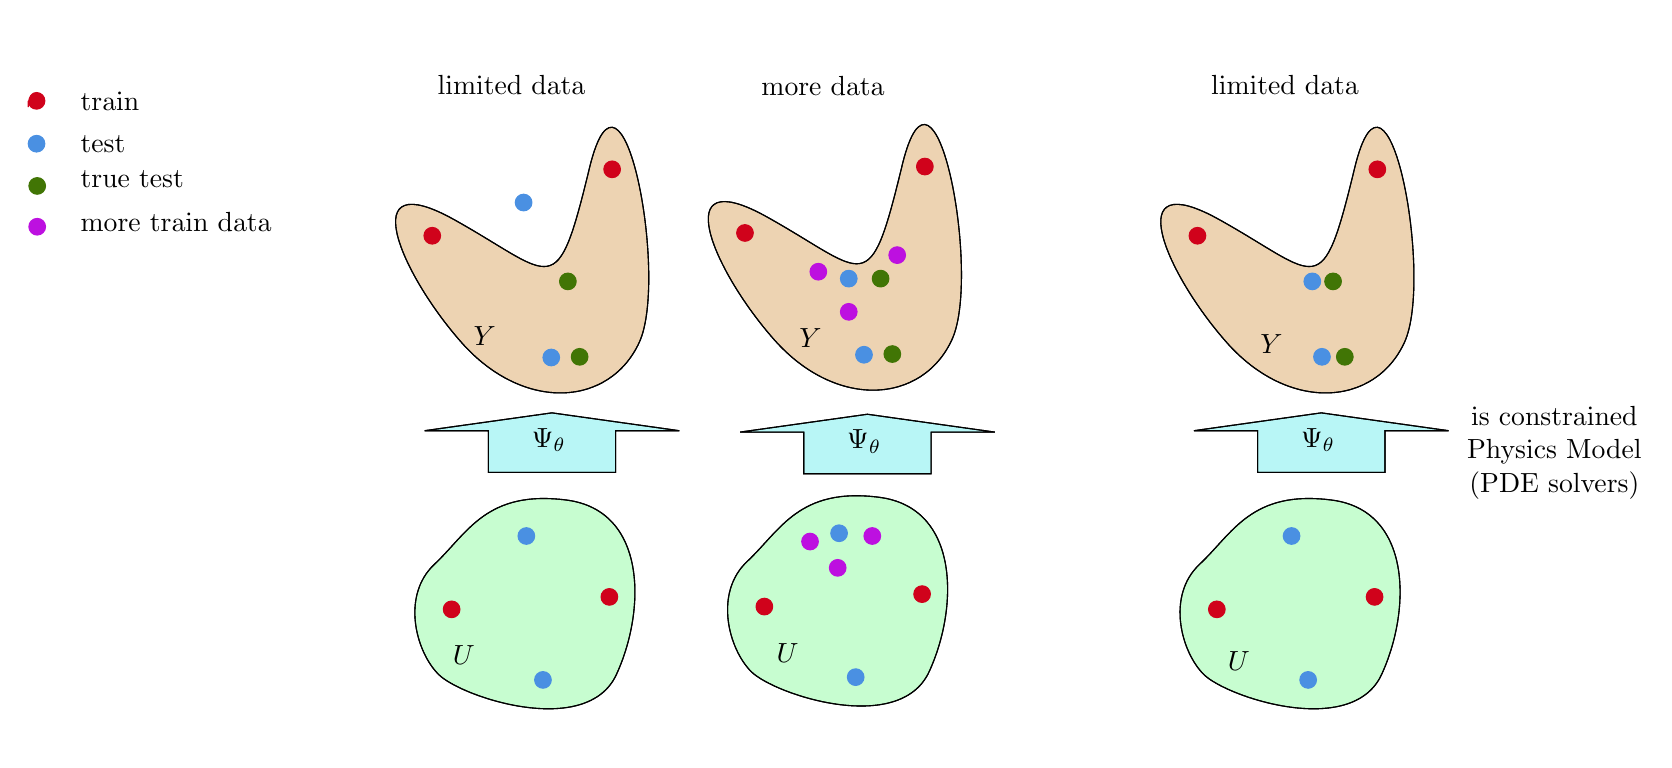
\begin{tikzpicture}[x=0.75pt,y=0.75pt,yscale=-1,xscale=1]
%uncomment if require: \path (0,500); %set diagram left start at 0, and has height of 500

%Shape: Polygon Curved [id:ds09447833398141592] 
\draw  [fill={rgb, 255:red, 197; green, 110; blue, 0 }  ,fill opacity=.3 ] (54.67,193) .. controls (24.67,159) and (3.15,107.04) .. (51.41,134.02) .. controls (99.67,161) and (100.41,175.02) .. (116.41,109.02) .. controls (132.41,43.02) and (154.67,162) .. (140.41,193.02) .. controls (126.15,224.04) and (84.67,227) .. (54.67,193) -- cycle ;
%Shape: Polygon Curved [id:ds8342971788940445] 
\draw  [fill={rgb, 255:red, 70; green, 248; blue, 100 }  ,fill opacity=.3 ] (43.67,353) .. controls (32.67,342) and (25.67,315) .. (41.67,300) .. controls (57.67,285) and (66.67,264) .. (105.41,269.02) .. controls (144.15,274.04) and (143.67,322) .. (129.41,353.02) .. controls (115.15,384.04) and (54.67,364) .. (43.67,353) -- cycle ;
%Shape: Polygon Curved [id:ds3279137678612456] 
\draw  [fill={rgb, 255:red, 197; green, 110; blue, 0 }  ,fill opacity=.3 ] (205.33,191.67) .. controls (175.33,157.67) and (153.82,105.7) .. (202.07,132.69) .. controls (250.33,159.67) and (251.07,173.69) .. (267.07,107.69) .. controls (283.07,41.69) and (305.33,160.67) .. (291.07,191.69) .. controls (276.82,222.7) and (235.33,225.67) .. (205.33,191.67) -- cycle ;
%Shape: Polygon Curved [id:ds20441696774386264] 
\draw  [fill={rgb, 255:red, 70; green, 248; blue, 100 }  ,fill opacity=.3 ] (194.33,351.67) .. controls (183.33,340.67) and (176.33,313.67) .. (192.33,298.67) .. controls (208.33,283.67) and (217.33,262.67) .. (256.07,267.69) .. controls (294.82,272.7) and (294.33,320.67) .. (280.07,351.69) .. controls (265.82,382.7) and (205.33,362.67) .. (194.33,351.67) -- cycle ;
%Shape: Polygon Curved [id:ds07726784585526025] 
\draw  [fill={rgb, 255:red, 197; green, 110; blue, 0 }  ,fill opacity=.3 ] (423.33,193) .. controls (393.33,159) and (371.82,107.04) .. (420.07,134.02) .. controls (468.33,161) and (469.07,175.02) .. (485.07,109.02) .. controls (501.07,43.02) and (523.33,162) .. (509.07,193.02) .. controls (494.82,224.04) and (453.33,227) .. (423.33,193) -- cycle ;
%Shape: Polygon Curved [id:ds010660115400260906] 
\draw  [fill={rgb, 255:red, 70; green, 248; blue, 100 }  ,fill opacity=.3 ] (412.33,353) .. controls (401.33,342) and (394.33,315) .. (410.33,300) .. controls (426.33,285) and (435.33,264) .. (474.07,269.02) .. controls (512.82,274.04) and (512.33,322) .. (498.07,353.02) .. controls (483.82,384.04) and (423.33,364) .. (412.33,353) -- cycle ;
%Up Arrow [id:dp6794269498576513] 
\draw  [fill={rgb, 255:red, 20; green, 225; blue, 225 }  ,fill opacity=.3 ] (37,235.6) -- (98.33,227) -- (159.67,235.6) -- (129,235.6) -- (129,255.67) -- (67.67,255.67) -- (67.67,235.6) -- cycle ;
%Up Arrow [id:dp09726735914616291] 
\draw  [fill={rgb, 255:red, 20; green, 225; blue, 225 }  ,fill opacity=.3 ] (189,236.27) -- (250.33,227.67) -- (311.67,236.27) -- (281,236.27) -- (281,256.33) -- (219.67,256.33) -- (219.67,236.27) -- cycle ;
%Up Arrow [id:dp5149313118072518] 
\draw  [fill={rgb, 255:red, 20; green, 225; blue, 225 }  ,fill opacity=.3 ] (407.67,235.6) -- (469,227) -- (530.33,235.6) -- (499.67,235.6) -- (499.67,255.67) -- (438.33,255.67) -- (438.33,235.6) -- cycle ;

%Shape: Polygon Curved [id:ds09447833398141592] 
\draw   (54.67,193) .. controls (24.67,159) and (3.15,107.04) .. (51.41,134.02) .. controls (99.67,161) and (100.41,175.02) .. (116.41,109.02) .. controls (132.41,43.02) and (154.67,162) .. (140.41,193.02) .. controls (126.15,224.04) and (84.67,227) .. (54.67,193) -- cycle ;
%Shape: Polygon Curved [id:ds8342971788940445] 
\draw   (43.67,353) .. controls (32.67,342) and (25.67,315) .. (41.67,300) .. controls (57.67,285) and (66.67,264) .. (105.41,269.02) .. controls (144.15,274.04) and (143.67,322) .. (129.41,353.02) .. controls (115.15,384.04) and (54.67,364) .. (43.67,353) -- cycle ;
%Shape: Circle [id:dp26432558400430295] 
\draw  [color={rgb, 255:red, 208; green, 2; blue, 27 }  ,draw opacity=1 ][fill={rgb, 255:red, 208; green, 2; blue, 27 }  ,fill opacity=1 ] (46,321.67) .. controls (46,319.46) and (47.79,317.67) .. (50,317.67) .. controls (52.21,317.67) and (54,319.46) .. (54,321.67) .. controls (54,323.88) and (52.21,325.67) .. (50,325.67) .. controls (47.79,325.67) and (46,323.88) .. (46,321.67) -- cycle ;
%Shape: Circle [id:dp7486480801214225] 
\draw  [color={rgb, 255:red, 208; green, 2; blue, 27 }  ,draw opacity=1 ][fill={rgb, 255:red, 208; green, 2; blue, 27 }  ,fill opacity=1 ] (122,315.67) .. controls (122,313.46) and (123.79,311.67) .. (126,311.67) .. controls (128.21,311.67) and (130,313.46) .. (130,315.67) .. controls (130,317.88) and (128.21,319.67) .. (126,319.67) .. controls (123.79,319.67) and (122,317.88) .. (122,315.67) -- cycle ;
%Shape: Circle [id:dp9817597880379183] 
\draw  [color={rgb, 255:red, 208; green, 2; blue, 27 }  ,draw opacity=1 ][fill={rgb, 255:red, 208; green, 2; blue, 27 }  ,fill opacity=1 ] (36.67,141.67) .. controls (36.67,139.46) and (38.46,137.67) .. (40.67,137.67) .. controls (42.88,137.67) and (44.67,139.46) .. (44.67,141.67) .. controls (44.67,143.88) and (42.88,145.67) .. (40.67,145.67) .. controls (38.46,145.67) and (36.67,143.88) .. (36.67,141.67) -- cycle ;
%Shape: Circle [id:dp006804475688651168] 
\draw  [color={rgb, 255:red, 208; green, 2; blue, 27 }  ,draw opacity=1 ][fill={rgb, 255:red, 208; green, 2; blue, 27 }  ,fill opacity=1 ] (123.33,109.67) .. controls (123.33,107.46) and (125.12,105.67) .. (127.33,105.67) .. controls (129.54,105.67) and (131.33,107.46) .. (131.33,109.67) .. controls (131.33,111.88) and (129.54,113.67) .. (127.33,113.67) .. controls (125.12,113.67) and (123.33,111.88) .. (123.33,109.67) -- cycle ;
%Shape: Circle [id:dp009892328190684307] 
\draw  [color={rgb, 255:red, 74; green, 144; blue, 226 }  ,draw opacity=1 ][fill={rgb, 255:red, 74; green, 144; blue, 226 }  ,fill opacity=1 ] (90,355.67) .. controls (90,353.46) and (91.79,351.67) .. (94,351.67) .. controls (96.21,351.67) and (98,353.46) .. (98,355.67) .. controls (98,357.88) and (96.21,359.67) .. (94,359.67) .. controls (91.79,359.67) and (90,357.88) .. (90,355.67) -- cycle ;
%Shape: Circle [id:dp3982721887803482] 
\draw  [color={rgb, 255:red, 74; green, 144; blue, 226 }  ,draw opacity=1 ][fill={rgb, 255:red, 74; green, 144; blue, 226 }  ,fill opacity=1 ] (82,286.33) .. controls (82,284.12) and (83.79,282.33) .. (86,282.33) .. controls (88.21,282.33) and (90,284.12) .. (90,286.33) .. controls (90,288.54) and (88.21,290.33) .. (86,290.33) .. controls (83.79,290.33) and (82,288.54) .. (82,286.33) -- cycle ;
%Shape: Circle [id:dp49175636396347844] 
\draw  [color={rgb, 255:red, 74; green, 144; blue, 226 }  ,draw opacity=1 ][fill={rgb, 255:red, 74; green, 144; blue, 226 }  ,fill opacity=1 ] (94,200.33) .. controls (94,198.12) and (95.79,196.33) .. (98,196.33) .. controls (100.21,196.33) and (102,198.12) .. (102,200.33) .. controls (102,202.54) and (100.21,204.33) .. (98,204.33) .. controls (95.79,204.33) and (94,202.54) .. (94,200.33) -- cycle ;
%Shape: Circle [id:dp21682181561205804] 
\draw  [color={rgb, 255:red, 74; green, 144; blue, 226 }  ,draw opacity=1 ][fill={rgb, 255:red, 74; green, 144; blue, 226 }  ,fill opacity=1 ] (80.67,125.67) .. controls (80.67,123.46) and (82.46,121.67) .. (84.67,121.67) .. controls (86.88,121.67) and (88.67,123.46) .. (88.67,125.67) .. controls (88.67,127.88) and (86.88,129.67) .. (84.67,129.67) .. controls (82.46,129.67) and (80.67,127.88) .. (80.67,125.67) -- cycle ;
%Shape: Circle [id:dp8907831670398318] 
\draw  [color={rgb, 255:red, 65; green, 117; blue, 5 }  ,draw opacity=1 ][fill={rgb, 255:red, 65; green, 117; blue, 5 }  ,fill opacity=1 ] (107.67,200) .. controls (107.67,197.79) and (109.46,196) .. (111.67,196) .. controls (113.88,196) and (115.67,197.79) .. (115.67,200) .. controls (115.67,202.21) and (113.88,204) .. (111.67,204) .. controls (109.46,204) and (107.67,202.21) .. (107.67,200) -- cycle ;
%Shape: Circle [id:dp5286507300103176] 
\draw  [color={rgb, 255:red, 65; green, 117; blue, 5 }  ,draw opacity=1 ][fill={rgb, 255:red, 65; green, 117; blue, 5 }  ,fill opacity=1 ] (102,163.67) .. controls (102,161.46) and (103.79,159.67) .. (106,159.67) .. controls (108.21,159.67) and (110,161.46) .. (110,163.67) .. controls (110,165.88) and (108.21,167.67) .. (106,167.67) .. controls (103.79,167.67) and (102,165.88) .. (102,163.67) -- cycle ;
%Shape: Polygon Curved [id:ds3279137678612456] 
\draw   (205.33,191.67) .. controls (175.33,157.67) and (153.82,105.7) .. (202.07,132.69) .. controls (250.33,159.67) and (251.07,173.69) .. (267.07,107.69) .. controls (283.07,41.69) and (305.33,160.67) .. (291.07,191.69) .. controls (276.82,222.7) and (235.33,225.67) .. (205.33,191.67) -- cycle ;
%Shape: Polygon Curved [id:ds20441696774386264] 
\draw   (194.33,351.67) .. controls (183.33,340.67) and (176.33,313.67) .. (192.33,298.67) .. controls (208.33,283.67) and (217.33,262.67) .. (256.07,267.69) .. controls (294.82,272.7) and (294.33,320.67) .. (280.07,351.69) .. controls (265.82,382.7) and (205.33,362.67) .. (194.33,351.67) -- cycle ;
%Shape: Circle [id:dp8376942440901165] 
\draw  [color={rgb, 255:red, 208; green, 2; blue, 27 }  ,draw opacity=1 ][fill={rgb, 255:red, 208; green, 2; blue, 27 }  ,fill opacity=1 ] (196.67,320.33) .. controls (196.67,318.12) and (198.46,316.33) .. (200.67,316.33) .. controls (202.88,316.33) and (204.67,318.12) .. (204.67,320.33) .. controls (204.67,322.54) and (202.88,324.33) .. (200.67,324.33) .. controls (198.46,324.33) and (196.67,322.54) .. (196.67,320.33) -- cycle ;
%Shape: Circle [id:dp6923958625920651] 
\draw  [color={rgb, 255:red, 208; green, 2; blue, 27 }  ,draw opacity=1 ][fill={rgb, 255:red, 208; green, 2; blue, 27 }  ,fill opacity=1 ] (272.67,314.33) .. controls (272.67,312.12) and (274.46,310.33) .. (276.67,310.33) .. controls (278.88,310.33) and (280.67,312.12) .. (280.67,314.33) .. controls (280.67,316.54) and (278.88,318.33) .. (276.67,318.33) .. controls (274.46,318.33) and (272.67,316.54) .. (272.67,314.33) -- cycle ;
%Shape: Circle [id:dp7389445208598843] 
\draw  [color={rgb, 255:red, 208; green, 2; blue, 27 }  ,draw opacity=1 ][fill={rgb, 255:red, 208; green, 2; blue, 27 }  ,fill opacity=1 ] (187.33,140.33) .. controls (187.33,138.12) and (189.12,136.33) .. (191.33,136.33) .. controls (193.54,136.33) and (195.33,138.12) .. (195.33,140.33) .. controls (195.33,142.54) and (193.54,144.33) .. (191.33,144.33) .. controls (189.12,144.33) and (187.33,142.54) .. (187.33,140.33) -- cycle ;
%Shape: Circle [id:dp09462367026507623] 
\draw  [color={rgb, 255:red, 208; green, 2; blue, 27 }  ,draw opacity=1 ][fill={rgb, 255:red, 208; green, 2; blue, 27 }  ,fill opacity=1 ] (274,108.33) .. controls (274,106.12) and (275.79,104.33) .. (278,104.33) .. controls (280.21,104.33) and (282,106.12) .. (282,108.33) .. controls (282,110.54) and (280.21,112.33) .. (278,112.33) .. controls (275.79,112.33) and (274,110.54) .. (274,108.33) -- cycle ;
%Shape: Circle [id:dp11319586275056814] 
\draw  [color={rgb, 255:red, 74; green, 144; blue, 226 }  ,draw opacity=1 ][fill={rgb, 255:red, 74; green, 144; blue, 226 }  ,fill opacity=1 ] (240.67,354.33) .. controls (240.67,352.12) and (242.46,350.33) .. (244.67,350.33) .. controls (246.88,350.33) and (248.67,352.12) .. (248.67,354.33) .. controls (248.67,356.54) and (246.88,358.33) .. (244.67,358.33) .. controls (242.46,358.33) and (240.67,356.54) .. (240.67,354.33) -- cycle ;
%Shape: Circle [id:dp8920361474219186] 
\draw  [color={rgb, 255:red, 74; green, 144; blue, 226 }  ,draw opacity=1 ][fill={rgb, 255:red, 74; green, 144; blue, 226 }  ,fill opacity=1 ] (232.67,285) .. controls (232.67,282.79) and (234.46,281) .. (236.67,281) .. controls (238.88,281) and (240.67,282.79) .. (240.67,285) .. controls (240.67,287.21) and (238.88,289) .. (236.67,289) .. controls (234.46,289) and (232.67,287.21) .. (232.67,285) -- cycle ;
%Shape: Circle [id:dp9966673763530642] 
\draw  [color={rgb, 255:red, 74; green, 144; blue, 226 }  ,draw opacity=1 ][fill={rgb, 255:red, 74; green, 144; blue, 226 }  ,fill opacity=1 ] (244.67,199) .. controls (244.67,196.79) and (246.46,195) .. (248.67,195) .. controls (250.88,195) and (252.67,196.79) .. (252.67,199) .. controls (252.67,201.21) and (250.88,203) .. (248.67,203) .. controls (246.46,203) and (244.67,201.21) .. (244.67,199) -- cycle ;
%Shape: Circle [id:dp3136076301608942] 
\draw  [color={rgb, 255:red, 74; green, 144; blue, 226 }  ,draw opacity=1 ][fill={rgb, 255:red, 74; green, 144; blue, 226 }  ,fill opacity=1 ] (237.33,162.33) .. controls (237.33,160.12) and (239.12,158.33) .. (241.33,158.33) .. controls (243.54,158.33) and (245.33,160.12) .. (245.33,162.33) .. controls (245.33,164.54) and (243.54,166.33) .. (241.33,166.33) .. controls (239.12,166.33) and (237.33,164.54) .. (237.33,162.33) -- cycle ;
%Shape: Circle [id:dp3648098032954873] 
\draw  [color={rgb, 255:red, 65; green, 117; blue, 5 }  ,draw opacity=1 ][fill={rgb, 255:red, 65; green, 117; blue, 5 }  ,fill opacity=1 ] (258.33,198.67) .. controls (258.33,196.46) and (260.12,194.67) .. (262.33,194.67) .. controls (264.54,194.67) and (266.33,196.46) .. (266.33,198.67) .. controls (266.33,200.88) and (264.54,202.67) .. (262.33,202.67) .. controls (260.12,202.67) and (258.33,200.88) .. (258.33,198.67) -- cycle ;
%Shape: Circle [id:dp512662669745621] 
\draw  [color={rgb, 255:red, 65; green, 117; blue, 5 }  ,draw opacity=1 ][fill={rgb, 255:red, 65; green, 117; blue, 5 }  ,fill opacity=1 ] (252.67,162.33) .. controls (252.67,160.12) and (254.46,158.33) .. (256.67,158.33) .. controls (258.88,158.33) and (260.67,160.12) .. (260.67,162.33) .. controls (260.67,164.54) and (258.88,166.33) .. (256.67,166.33) .. controls (254.46,166.33) and (252.67,164.54) .. (252.67,162.33) -- cycle ;
%Shape: Circle [id:dp5844049985343532] 
\draw  [color={rgb, 255:red, 189; green, 16; blue, 224 }  ,draw opacity=1 ][fill={rgb, 255:red, 189; green, 16; blue, 224 }  ,fill opacity=1 ] (218.67,289) .. controls (218.67,286.79) and (220.46,285) .. (222.67,285) .. controls (224.88,285) and (226.67,286.79) .. (226.67,289) .. controls (226.67,291.21) and (224.88,293) .. (222.67,293) .. controls (220.46,293) and (218.67,291.21) .. (218.67,289) -- cycle ;
%Shape: Circle [id:dp21392691792594376] 
\draw  [color={rgb, 255:red, 189; green, 16; blue, 224 }  ,draw opacity=1 ][fill={rgb, 255:red, 189; green, 16; blue, 224 }  ,fill opacity=1 ] (248.67,286.33) .. controls (248.67,284.12) and (250.46,282.33) .. (252.67,282.33) .. controls (254.88,282.33) and (256.67,284.12) .. (256.67,286.33) .. controls (256.67,288.54) and (254.88,290.33) .. (252.67,290.33) .. controls (250.46,290.33) and (248.67,288.54) .. (248.67,286.33) -- cycle ;
%Shape: Circle [id:dp03765555278678889] 
\draw  [color={rgb, 255:red, 189; green, 16; blue, 224 }  ,draw opacity=1 ][fill={rgb, 255:red, 189; green, 16; blue, 224 }  ,fill opacity=1 ] (222.67,159) .. controls (222.67,156.79) and (224.46,155) .. (226.67,155) .. controls (228.88,155) and (230.67,156.79) .. (230.67,159) .. controls (230.67,161.21) and (228.88,163) .. (226.67,163) .. controls (224.46,163) and (222.67,161.21) .. (222.67,159) -- cycle ;
%Shape: Circle [id:dp3713963754985672] 
\draw  [color={rgb, 255:red, 189; green, 16; blue, 224 }  ,draw opacity=1 ][fill={rgb, 255:red, 189; green, 16; blue, 224 }  ,fill opacity=1 ] (260.67,151) .. controls (260.67,148.79) and (262.46,147) .. (264.67,147) .. controls (266.88,147) and (268.67,148.79) .. (268.67,151) .. controls (268.67,153.21) and (266.88,155) .. (264.67,155) .. controls (262.46,155) and (260.67,153.21) .. (260.67,151) -- cycle ;
%Shape: Circle [id:dp4867530767856524] 
\draw  [color={rgb, 255:red, 189; green, 16; blue, 224 }  ,draw opacity=1 ][fill={rgb, 255:red, 189; green, 16; blue, 224 }  ,fill opacity=1 ] (232,301.67) .. controls (232,299.46) and (233.79,297.67) .. (236,297.67) .. controls (238.21,297.67) and (240,299.46) .. (240,301.67) .. controls (240,303.88) and (238.21,305.67) .. (236,305.67) .. controls (233.79,305.67) and (232,303.88) .. (232,301.67) -- cycle ;
%Shape: Circle [id:dp26156864275097613] 
\draw  [color={rgb, 255:red, 189; green, 16; blue, 224 }  ,draw opacity=1 ][fill={rgb, 255:red, 189; green, 16; blue, 224 }  ,fill opacity=1 ] (237.33,178.33) .. controls (237.33,176.12) and (239.12,174.33) .. (241.33,174.33) .. controls (243.54,174.33) and (245.33,176.12) .. (245.33,178.33) .. controls (245.33,180.54) and (243.54,182.33) .. (241.33,182.33) .. controls (239.12,182.33) and (237.33,180.54) .. (237.33,178.33) -- cycle ;
%Shape: Polygon Curved [id:ds07726784585526025] 
\draw   (423.33,193) .. controls (393.33,159) and (371.82,107.04) .. (420.07,134.02) .. controls (468.33,161) and (469.07,175.02) .. (485.07,109.02) .. controls (501.07,43.02) and (523.33,162) .. (509.07,193.02) .. controls (494.82,224.04) and (453.33,227) .. (423.33,193) -- cycle ;
%Shape: Polygon Curved [id:ds010660115400260906] 
\draw   (412.33,353) .. controls (401.33,342) and (394.33,315) .. (410.33,300) .. controls (426.33,285) and (435.33,264) .. (474.07,269.02) .. controls (512.82,274.04) and (512.33,322) .. (498.07,353.02) .. controls (483.82,384.04) and (423.33,364) .. (412.33,353) -- cycle ;
%Shape: Circle [id:dp6050150972945199] 
\draw  [color={rgb, 255:red, 208; green, 2; blue, 27 }  ,draw opacity=1 ][fill={rgb, 255:red, 208; green, 2; blue, 27 }  ,fill opacity=1 ] (414.67,321.67) .. controls (414.67,319.46) and (416.46,317.67) .. (418.67,317.67) .. controls (420.88,317.67) and (422.67,319.46) .. (422.67,321.67) .. controls (422.67,323.88) and (420.88,325.67) .. (418.67,325.67) .. controls (416.46,325.67) and (414.67,323.88) .. (414.67,321.67) -- cycle ;
%Shape: Circle [id:dp9364297613608107] 
\draw  [color={rgb, 255:red, 208; green, 2; blue, 27 }  ,draw opacity=1 ][fill={rgb, 255:red, 208; green, 2; blue, 27 }  ,fill opacity=1 ] (490.67,315.67) .. controls (490.67,313.46) and (492.46,311.67) .. (494.67,311.67) .. controls (496.88,311.67) and (498.67,313.46) .. (498.67,315.67) .. controls (498.67,317.88) and (496.88,319.67) .. (494.67,319.67) .. controls (492.46,319.67) and (490.67,317.88) .. (490.67,315.67) -- cycle ;
%Shape: Circle [id:dp23887389693118888] 
\draw  [color={rgb, 255:red, 208; green, 2; blue, 27 }  ,draw opacity=1 ][fill={rgb, 255:red, 208; green, 2; blue, 27 }  ,fill opacity=1 ] (405.33,141.67) .. controls (405.33,139.46) and (407.12,137.67) .. (409.33,137.67) .. controls (411.54,137.67) and (413.33,139.46) .. (413.33,141.67) .. controls (413.33,143.88) and (411.54,145.67) .. (409.33,145.67) .. controls (407.12,145.67) and (405.33,143.88) .. (405.33,141.67) -- cycle ;
%Shape: Circle [id:dp6245898218338471] 
\draw  [color={rgb, 255:red, 208; green, 2; blue, 27 }  ,draw opacity=1 ][fill={rgb, 255:red, 208; green, 2; blue, 27 }  ,fill opacity=1 ] (492,109.67) .. controls (492,107.46) and (493.79,105.67) .. (496,105.67) .. controls (498.21,105.67) and (500,107.46) .. (500,109.67) .. controls (500,111.88) and (498.21,113.67) .. (496,113.67) .. controls (493.79,113.67) and (492,111.88) .. (492,109.67) -- cycle ;
%Shape: Circle [id:dp9009813115521121] 
\draw  [color={rgb, 255:red, 74; green, 144; blue, 226 }  ,draw opacity=1 ][fill={rgb, 255:red, 74; green, 144; blue, 226 }  ,fill opacity=1 ] (458.67,355.67) .. controls (458.67,353.46) and (460.46,351.67) .. (462.67,351.67) .. controls (464.88,351.67) and (466.67,353.46) .. (466.67,355.67) .. controls (466.67,357.88) and (464.88,359.67) .. (462.67,359.67) .. controls (460.46,359.67) and (458.67,357.88) .. (458.67,355.67) -- cycle ;
%Shape: Circle [id:dp5708756535513383] 
\draw  [color={rgb, 255:red, 74; green, 144; blue, 226 }  ,draw opacity=1 ][fill={rgb, 255:red, 74; green, 144; blue, 226 }  ,fill opacity=1 ] (450.67,286.33) .. controls (450.67,284.12) and (452.46,282.33) .. (454.67,282.33) .. controls (456.88,282.33) and (458.67,284.12) .. (458.67,286.33) .. controls (458.67,288.54) and (456.88,290.33) .. (454.67,290.33) .. controls (452.46,290.33) and (450.67,288.54) .. (450.67,286.33) -- cycle ;
%Shape: Circle [id:dp5227952073213964] 
\draw  [color={rgb, 255:red, 74; green, 144; blue, 226 }  ,draw opacity=1 ][fill={rgb, 255:red, 74; green, 144; blue, 226 }  ,fill opacity=1 ] (465.33,200) .. controls (465.33,197.79) and (467.12,196) .. (469.33,196) .. controls (471.54,196) and (473.33,197.79) .. (473.33,200) .. controls (473.33,202.21) and (471.54,204) .. (469.33,204) .. controls (467.12,204) and (465.33,202.21) .. (465.33,200) -- cycle ;
%Shape: Circle [id:dp8422423939560267] 
\draw  [color={rgb, 255:red, 74; green, 144; blue, 226 }  ,draw opacity=1 ][fill={rgb, 255:red, 74; green, 144; blue, 226 }  ,fill opacity=1 ] (460.67,163.67) .. controls (460.67,161.46) and (462.46,159.67) .. (464.67,159.67) .. controls (466.88,159.67) and (468.67,161.46) .. (468.67,163.67) .. controls (468.67,165.88) and (466.88,167.67) .. (464.67,167.67) .. controls (462.46,167.67) and (460.67,165.88) .. (460.67,163.67) -- cycle ;
%Shape: Circle [id:dp3798294341721118] 
\draw  [color={rgb, 255:red, 65; green, 117; blue, 5 }  ,draw opacity=1 ][fill={rgb, 255:red, 65; green, 117; blue, 5 }  ,fill opacity=1 ] (476.33,200) .. controls (476.33,197.79) and (478.12,196) .. (480.33,196) .. controls (482.54,196) and (484.33,197.79) .. (484.33,200) .. controls (484.33,202.21) and (482.54,204) .. (480.33,204) .. controls (478.12,204) and (476.33,202.21) .. (476.33,200) -- cycle ;
%Shape: Circle [id:dp8266340050542115] 
\draw  [color={rgb, 255:red, 65; green, 117; blue, 5 }  ,draw opacity=1 ][fill={rgb, 255:red, 65; green, 117; blue, 5 }  ,fill opacity=1 ] (470.67,163.67) .. controls (470.67,161.46) and (472.46,159.67) .. (474.67,159.67) .. controls (476.88,159.67) and (478.67,161.46) .. (478.67,163.67) .. controls (478.67,165.88) and (476.88,167.67) .. (474.67,167.67) .. controls (472.46,167.67) and (470.67,165.88) .. (470.67,163.67) -- cycle ;
%Up Arrow [id:dp6794269498576513] 
\draw   (37,235.6) -- (98.33,227) -- (159.67,235.6) -- (129,235.6) -- (129,255.67) -- (67.67,255.67) -- (67.67,235.6) -- cycle ;
%Up Arrow [id:dp09726735914616291] 
\draw   (189,236.27) -- (250.33,227.67) -- (311.67,236.27) -- (281,236.27) -- (281,256.33) -- (219.67,256.33) -- (219.67,236.27) -- cycle ;
%Up Arrow [id:dp5149313118072518] 
\draw   (407.67,235.6) -- (469,227) -- (530.33,235.6) -- (499.67,235.6) -- (499.67,255.67) -- (438.33,255.67) -- (438.33,235.6) -- cycle ;


% Text Node
\draw (42,60 + 3) node [anchor=north west][inner sep=0.75pt]   [align=left] {limited data};
% Text Node
\draw (198,60.67 + 3) node [anchor=north west][inner sep=0.75pt]   [align=left] {more data};
% Text Node
\draw (414.67,60.33 + 3) node [anchor=north west][inner sep=0.75pt]   [align=left] {limited data};
% Text Node
\draw (538,219.67 + 3) node [anchor=north west][inner sep=0.75pt]   [align=center] {is constrained\\Physics Model \\ (PDE solvers)};
% Text Node
\draw (87.33,230.33 + 3) node [anchor=north west][inner sep=0.75pt]    {$\Psi _{\theta }$};
% Text Node
\draw (239.33,231 + 3) node [anchor=north west][inner sep=0.75pt]    {$\Psi _{\theta }$};
% Text Node
\draw (458,230.33 + 3) node [anchor=north west][inner sep=0.75pt]    {$\Psi _{\theta }$};
% Text Node
\draw (49.33,335 + 3) node [anchor=north west][inner sep=0.75pt]    {$U$};
% Text Node
\draw (205.33,333.67 + 3) node [anchor=north west][inner sep=0.75pt]    {$U$};
% Text Node
\draw (422.67,337.67 + 3) node [anchor=north west][inner sep=0.75pt]    {$U$};
% Text Node
\draw (59.33,181 + 3) node [anchor=north west][inner sep=0.75pt]    {$Y$};
% Text Node
\draw (216.33,182.33 + 3) node [anchor=north west][inner sep=0.75pt]    {$Y$};
% Text Node
\draw (438.33,185 + 3) node [anchor=north west][inner sep=0.75pt]    {$Y$};

% Text Node
\draw (-130,449 - 320) node [anchor=north west][inner sep=0.75pt]   [align=left] {more train data};
% Text Node
\draw (-130,429 - 320) node [anchor=north west][inner sep=0.75pt]   [align=left] {true test};
% Text Node
\draw (-130,409.- 320 +3) node [anchor=north west][inner sep=0.75pt]   [align=left] {test};
% Text Node
\draw (-130,388.- 320 +3) node [anchor=north west][inner sep=0.75pt]   [align=left] {train};

%Shape: Circle [id:dp6233320255874407]
\draw [color={rgb, 255:red, 208; green, 2; blue, 27 } ,draw opacity=1 ][fill={rgb, 255:red, 208; green, 2; blue, 27 } ,fill opacity=1 ] (66-220,399.67-320) .. controls (66-220,397.46-320+-3) and (67.79-220,395.67-320+-3) .. (70-220,395.67-320+-3) .. controls (72.21-220,395.67-320+-3) and (74-220,397.46-320+-3) .. (74-220,399.67-320+-3) .. controls (74-220,401.88-320+-3) and (72.21-220,403.67-320+-3) .. (70-220,403.67-320+-3) .. controls (67.79-220,403.67-320+-3) and (66-220,401.88-320+-3) .. (66-220,399.67-320+-3) -- cycle ;
%Shape: Circle [id:dp4869712809146013]
\draw [color={rgb, 255:red, 74; green, 144; blue, 226 } ,draw opacity=1 ][fill={rgb, 255:red, 74; green, 144; blue, 226 } ,fill opacity=1 ] (66-220,420.33-320+-3) .. controls (66-220,418.12-320+-3) and (67.79-220,416.33-320+-3) .. (70-220,416.33-320+-3) .. controls (72.21-220,416.33-320+-3) and (74-220,418.12-320+-3) .. (74-220,420.33-320+-3) .. controls (74-220,422.54-320+-3) and (72.21-220,424.33-320+-3) .. (70-220,424.33-320+-3) .. controls (67.79-220,424.33-320+-3) and (66-220,422.54-320+-3) .. (66-220,420.33-320+-3) -- cycle ;
%Shape: Circle [id:dp2109728352746062]
\draw [color={rgb, 255:red, 189; green, 16; blue, 224 } ,draw opacity=1 ][fill={rgb, 255:red, 189; green, 16; blue, 224 } ,fill opacity=1 ] (66.33-220,460.33-320+-3) .. controls (66.33-220,458.12-320+-3) and (68.12-220,456.33-320+-3) .. (70.33-220,456.33-320+-3) .. controls (72.54-220,456.33-320+-3) and (74.33-220,458.12-320+-3) .. (74.33-220,460.33-320+-3) .. controls (74.33-220,462.54-320+-3) and (72.54-220,464.33-320+-3) .. (70.33-220,464.33-320+-3) .. controls (68.12-220,464.33-320+-3) and (66.33-220,462.54-320+-3) .. (66.33-220,460.33-320+-3) -- cycle ;
%Shape: Circle [id:dp7961183108885519]
\draw [color={rgb, 255:red, 65; green, 117; blue, 5 } ,draw opacity=1 ][fill={rgb, 255:red, 65; green, 117; blue, 5 } ,fill opacity=1 ] (66.33-220,440.67-320+-3) .. controls (66.33-220,438.46-320+-3) and (68.12-220,436.67-320+-3) .. (70.33-220,436.67-320+-3) .. controls (72.54-220,436.67-320+-3) and (74.33-220,438.46-320+-3) .. (74.33-220,440.67-320+-3) .. controls (74.33-220,442.88-320+-3) and (72.54-220,444.67-320+-3) .. (70.33-220,444.67-320+-3) .. controls (68.12-220,444.67-320+-3) and (66.33-220,442.88-320+-3) .. (66.33-220,440.67-320+-3) -- cycle ;

\end{tikzpicture}

}


}}

% \frame{
\frametitle{Model-constrained Machine Learning for Solving Forward Problems}
% \vspace{-10ex}
\bluebox{I proposed two approaches:}
{    
\begin{itemize}
    \item \texttt{mcTangent} [\myblue{2}] for solving PDEs with smooth solutions.
    \item \texttt{DGNet} [\myblue{1}], an extension of \texttt{mcTangent}, for solving PDEs with discontinuous solutions.
\end{itemize}
}

\vspace{3ex}

{ \tiny
[1] {\bf H.V. Nguyen}, et. al. {\it ``A model-constrained Discontinuous Galerkin Network (DGNet) for Compressible Euler Equations with
Out-of-Distribution Generalization."} \newline
\vspace{-1ex}
$\quad $  Computer Methods in Applied Mechanics and Engineering (2025) 

[2] {\bf H.V. Nguyen}, et. al. {\it ``A Model-Constrained Tangent Slope Learning Approach for Dynamical Systems."} International Journal of
Computational Fluid Dynamics (2022)
}

}}
% \frame{
\frametitle{PDEs - General Dynamical Systems}
% \vspace{-10ex}
\bluebox{PDEs - System of conversation laws}
{    
    \begin{equation*}
        \begin{aligned}
            \pp{\ub}{t}\LRp{\xb,t} + \nabla \cdot \fb \LRp{\ub\LRp{\xb,t}} & = 0, & & \xb \in \Omega, t \in \LRs{0,T},\\
            \ub\LRp{\xb,t} & = \ub_{bc}\LRp{\xb,t}, & & \xb \in \partial \Omega,   t \in \LRs{0,T},\\
            \ub\LRp{\xb,0} & = \ub_0\LRp{\xb} , & & \xb \in \Omega.
        \end{aligned}
    \end{equation*}

can be rewritten in general dynamical system form as

\[
    \frac{d}{dt}\ub(\xb,t) = \mathcal{F}\LRp{\ub(\xb,t)}
\]

can be solved with the method of line. However, evaluation of $\mathcal{F}$ is {\bf computationally expensive.}

}

}}
% \frame{
\frametitle{Motivation}
% \vspace{-10ex}
\small
\bluebox{Common machine learning approaches for solving PDEs}
{    

\begin{itemize}
\item PINN [\myblue{Raissi M., 2019}]: solving for a case of dynamical
\item Transformer [\myblue{Li Zijie, 2024}], Graph neural network [\myblue{Iakovlev, V. 2020}]: capturing spatial/temporal correlations at once directly mapping from $T_i$ to $T_{i+1}$
\item Operator learning: FNO [\myblue{Li Z., 2020}], DeepONet [\myblue{Lu Lu, 2019}] directly mapping solutions from $T_0$ to $T_{end}$
\item Neural ODE [\myblue{Chen, R. T., 2018}]/Recurrent neural network [\myblue{Mohajerin, N. 2019}] (most related to our work) learning right hand side (tangent slope/dynamical evolution) of dynamical systems, temporal correlation is taken into consideration by time integration scheme.

\end{itemize}

}

\vspace{1ex}

\orangebox{Limitations}
{
    \begin{itemize}
        \item Inference stability, long-term prediction capacity due to inference error accumulation.
        \item Generalization to different scenarios (boundary conditions, geometry, invariant-discretization, ...)
        \item Discontinuities/shocks evolution (limited research)
    \end{itemize}
}

}}
% \frame{
\frametitle{Methodology - Key idea}
% \vspace{-10ex}
\small
\bluebox{Key idea}
{    

\begin{enumerate}
\item We design a time-invariant surrogate model, $\myblue{\Psi} \LRp{\cdot}$, to approximate the RHS, $\F \LRp{\cdot}$, of the dynamical system

$$\frac{d}{dt}\ub(\xb,t) = \F\LRp{\ub(\xb,t)}.$$

\item Once trained, we can use $\myblue{\Psi} \LRp{\cdot}$ to solve  

\[
    \frac{d}{dt}\ub(\xb,t) = \myblue{\Psi}\LRp{\ub(\xb,t)}.
\]

efficiently either with explicit or implicit time integration schemes.

\end{enumerate}

}

}

}
% \frame{\frametitle{\texttt{mcTangent}}
\framesubtitle{Naive machine learning}
\vspace{-6ex}
\bluebox{Consider forward Euler with the exact and approximate tangent slopes}{
    \[
        \ui{i+1} = \ui{i} + \dt \, \F \LRp{\ui{i}}, \quad \textcolor{green}{\ut{i+1}} = \ut{i} + \dt \NN{\ut{i}},
    \]
}
    \vspace{2ex}
    
    \orangebox{Training with naive machine learning}{
        \begin{itemize}
            \item Learn the tangent slope $\F$
                  \[
                      \textcolor{green}{\ut{i+1}} = \ut{i} + \dt \NN{\ut{i}},
                  \]
                  % Forward Euler scheme takes care temporal evolution. Network approximates tangent slope (spatial derivatives) only.
                  by  minimizing $\MSE{\textcolor{green}{\ut{i+1}} - \ui{i+1}}$.
        \end{itemize}
    }
}


}
% \frame{\frametitle{\texttt{mcTangent}}
    \framesubtitle{Model-constrained tangent slope learning approach}

    \bluebox{Consider forward Euler with the exact and approximate tangent slopes}{
        \[
            \ui{i+1} = \ui{i} + \dt \, \F \LRp{\ui{i}}, \quad \textcolor{green}{\ut{i+1}} = \ut{i} + \dt \NN{\ut{i}},
        \]
    }
    % \pause
    \vspace{2ex}
    \bluebox{Force machine learning predictions to satisfy the discretized equation}{
        %Two consecutive snapshots are constrained to satisfied the governed equation (True Forward-Euler scheme) by
        \begin{equation*}
            \begin{aligned}
                \frac{\textcolor{green}{\ut{i+1}} - \ut{i}}{\dt}                          & = \F \LRp{\ut{i}}                                                           \\
                                                                                          & \Updownarrow                                                                \\
                \underbrace{\ut{i} + \dt \Psi \LRp{\ut{i}}}_{\textcolor{green}{\ut{i+1}}} & = \underbrace{\ut{i} + \dt \F \LRp{\ut{i}}}_{\textcolor{blue}{\ubar{i+1}}}.
            \end{aligned}
        \end{equation*}
        \myred{In practice} we approximately accomplish this  by minimizing $\MSE{\textcolor{green}{\ut{i+1}} - \textcolor{blue}{\ubar{i+1}}}$
    }
}


}
% \input{\fromroot{slides/Forward_mcTangent_Euler_2.tex}}
% \frame{\frametitle{Schematic of \texttt{mcTangent}}
% \bluebox{Architecture}
{
    \def\layersep{2cm}
    \def\nodeinlayersep{.9cm}
    \usetikzlibrary{calc}
    
    \begin{figure}[htb!]
    \centering
    \begin{tikzpicture}[
        node distance=\layersep,
        edge/.style={-stealth,shorten >=1pt, draw=black!50,thin},
        neuron/.style={circle,fill=black!25,minimum size=10pt,inner sep=0pt},
        operator/.style={rectangle,fill=green!,minimum height= \nodeinlayersep, minimum width= 0.8 * \layersep, inner sep=0pt, rounded corners},
        input neuron/.style={neuron, fill=green!50,minimum size=12pt},
        output neuron/.style={neuron, fill=green!50,minimum size=12pt},
        hidden neuron/.style={neuron, fill=blue!50},
        Forward map/.style={operator, fill=red!50},
        annot/.style={text width=4em, text centered},
        every node/.style={scale=1.0},
        node1/.style={scale=2.0},
        cross/.style={path picture={ \draw[black, shorten <=2pt, shorten >=2pt, line width=1pt] (path picture bounding box.south) -- (path picture bounding box.north); \draw[black, shorten <=2pt, shorten >=2pt, line width=1pt] (path picture bounding box.west) -- (path picture bounding box.east);}}
    ]
    
    \node[rectangle,fill=yellow!50,minimum height= \nodeinlayersep, minimum width= 0.8 * \layersep, rounded corners] (u_in) at (0*\layersep, -2*\nodeinlayersep) {$\ui{{i,0}} + \epsb$};
    \node[rectangle,fill=yellow!50,minimum height= \nodeinlayersep, minimum width= 0.8 * \layersep, rounded corners] (u_ml_1) at (3.0*\layersep, -2*\nodeinlayersep) {$\ut{{i,1}}$};
    \node[rectangle,fill=yellow!50,minimum height= \nodeinlayersep, minimum width= 0.8 * \layersep, rounded corners] (u_ml_2) at (6.0*\layersep, -2*\nodeinlayersep) {$\ut{{i,2}}$};
    % \node[rectangle,fill=yellow!500,minimum height= \nodeinlayersep, minimum width= 0.5 * \layersep, rounded corners] (u_ml_3) at (7.*\layersep, -2*\nodeinlayersep) {$\hdots$};
    
    
    \node[rectangle,fill=blue!50,minimum height= \nodeinlayersep, minimum width= 0.8 * \layersep, rounded corners] (NN1) at (1.25*\layersep, -2*\nodeinlayersep) {$\Psi$};
    \node[rectangle,fill=blue!50,minimum height= \nodeinlayersep, minimum width= 0.8 * \layersep, rounded corners] (NN2) at (4.25*\layersep, -2*\nodeinlayersep) {$\Psi$};
    
    \node[rectangle,minimum height= \nodeinlayersep, minimum width= 0.8 * \layersep, rounded corners] (dt) at (1.9*\layersep, -1.8*\nodeinlayersep) {\tiny $ \times \dt$};
    
    \node[rectangle,minimum height= \nodeinlayersep, minimum width= 0.8 * \layersep, rounded corners] (dt) at (4.9*\layersep, -1.8*\nodeinlayersep) {\tiny $ \times \dt$};
    
    \node [draw,circle,cross,minimum width=.02*\layersep,line width=.3pt](cross_1) at (2.3*\layersep, -2*\nodeinlayersep){}; 
    \node [draw,circle,cross,minimum width=.1*\layersep,line width=.3pt](cross_2) at (5.3*\layersep, -2*\nodeinlayersep){};
    % \node [draw,circle,cross,minimum width=.1*\layersep,line width=.3pt](cross_3) at (5.2*\layersep, -4*\nodeinlayersep){};
    
    \node[rectangle,fill=red!50,minimum height= \nodeinlayersep, minimum width= 0.8 * \layersep, rounded corners] (forward_1) at (1.0*\layersep, -4*\nodeinlayersep) {$\mc{F}$};
    \node[rectangle,fill=yellow!50,minimum height= \nodeinlayersep, minimum width= 0.8 * \layersep, rounded corners] (u_mc_1) at (2.3*\layersep, -4*\nodeinlayersep) {$\ubar{{i,1}}$};
    
    \node[rectangle,fill=red!50,minimum height= \nodeinlayersep, minimum width= 0.8 * \layersep, rounded corners] (forward) at (4.0*\layersep, -4*\nodeinlayersep) {$\mc{F}$};
    \node[rectangle,fill=yellow!50,minimum height= \nodeinlayersep, minimum width= 0.8 * \layersep, rounded corners] (u_mc) at (5.3*\layersep, -4*\nodeinlayersep) {$\ubar{{i,2}}$};
    
    % \node[rectangle,fill=yellow!50,minimum height= \nodeinlayersep, minimum width= 0.8 * \layersep, rounded corners] (u_mc_2) at (8.0*\layersep, -4*\nodeinlayersep) {$\ubar{{j+2}}$};
    
    \draw[edge,thin] (u_in) -- (NN1);
    \draw[edge,thin] (NN1) -- (cross_1);
    \draw[edge,thin] (cross_1) -- (u_ml_1);
    \draw[edge,thin] (u_ml_1) -- (NN2);
    \draw[edge,thin] (NN2) -- (cross_2);
    \draw[edge,thin] (cross_2) -- (u_ml_2);
    % \draw[edge,thin] (u_ml_2) -- (u_ml_3);
    % \draw[edge,thin] (forward) -- (cross_3);
    % \draw[edge,thin] (cross_3) -- (u_mc);
    
    
    \draw[edge,thin] (.6*\layersep, -2*\nodeinlayersep) -- (.6*\layersep, -1.*\nodeinlayersep) -- (2.3*\layersep, -1.*\nodeinlayersep) -- (cross_1);
    
    \draw[edge,thin] (3.6*\layersep, -2*\nodeinlayersep) -- (3.6*\layersep, -1.*\nodeinlayersep) -- (5.3*\layersep, -1.*\nodeinlayersep) -- (cross_2);
    
    \draw[edge,thin] (u_in) -- (0.0*\layersep, -4.*\nodeinlayersep) -- (forward_1);
    \draw[edge,thin] (forward_1) -- (u_mc_1);
    
    \draw[edge,thin] (u_ml_1) -- (3.0*\layersep, -4.*\nodeinlayersep) -- (forward);
    \draw[edge,thin] (forward) -- (u_mc);
    
    
    
    % LOSS ML TERMS
    \node[rectangle,fill=green!40,minimum height= \nodeinlayersep, minimum width= 3.4 * \layersep, rounded corners] (loss_ml) at (4.5*\layersep, .6*\nodeinlayersep) {Loss $\mc{L}_n$: $ \MSE{\ui{{i,1}} - \ut{{i,1}}} +  \MSE{\ui{{i,2}} - \ut{{i,2}}}$};
    
    \node[rectangle,fill=green!0,minimum height= \nodeinlayersep, minimum width= 3.4 * \layersep, rounded corners] (loss_ml) at (1*\layersep, 1*\nodeinlayersep) {Considering $i$th dataset window};
    
    \node[rectangle,fill=green!0,minimum height= \nodeinlayersep, minimum width= 3.4 * \layersep, rounded corners] (loss_ml) at (1*\layersep, 0.3*\nodeinlayersep) {$\LRp{\ui{{i,0}}, \ui{{i,1}}, \ui{{i,2}}}$};
    
    
    
    \draw[edge,thin] (u_ml_1) -- (3.0*\layersep, .5*\nodeinlayersep - 0.4*\nodeinlayersep);
    \draw[edge,thin] (u_ml_2) -- (6.0*\layersep, .5*\nodeinlayersep - 0.4*\nodeinlayersep);
    
    % LOSS MC TERMS
    \node[rectangle,fill=green!40,minimum height= \nodeinlayersep, minimum width= 1.6 * \layersep, rounded corners] (loss_mc) at (3.0*\layersep, -6.0*\nodeinlayersep) {Loss $\mc{L}_{mc}$: $\alpha \MSE{ \ubar{{i,1}} - \ut{{i,1}}} + \MSE{ \ubar{{i,2}} - \ut{{i,2}}}$};
    % \draw[edge,thin] (u_ml_1) -- (3.0*\layersep, .5*\nodeinlayersep - 0.5*\nodeinlayersep);
    
    \draw[edge,thin] (2.95*\layersep, -2.5*\nodeinlayersep) -- (2.95*\layersep, -5.5*\nodeinlayersep);
    \draw[edge,thin] (u_mc_1) -- (2.95*\layersep, -4.0*\nodeinlayersep) -- (2.95*\layersep, -5.5*\nodeinlayersep);
    
    \draw[edge,thin] (u_ml_2) -- (6.0*\layersep, -6.0*\nodeinlayersep) -- (loss_mc);
    \draw[edge,thin] (u_mc) -- (6.0*\layersep, -4*\nodeinlayersep) -- (6.0*\layersep, -6.0*\nodeinlayersep) -- (loss_mc);
    
        
    \end{tikzpicture}
    \end{figure}
}
}
}
% \frame{\frametitle{Analysis: Data randomization}
    % \bluebox{randomized inputs}{
    % \[\ubr = \ub + \epsb,\]
    % where $\epsb$ is a normal random vector $\epsb \sim \mc{N}\LRp{\bs{0}, \delta^2 \Ib}$
    % }

\bluebox{Loss function (sum over all dataset windows)}{
\[
\mc{L} := \frac{1}{N_t} \sum_{i=0}^{N_t - 1} \MSE{\ui{i,1} - \ut{i,1}} + \alpha \MSE{\ubar{i,1} - \ut{i,1}}
\]
}

\vspace{2ex}

\orangebox{Randomized loss function}{
    Denoting randomized version of $\ui{i,0}$ is
    \begin{equation*}
        \vi{i,0} = \ui{i,0} + \epsb
    \end{equation*}
    where, $\epsb$ is noise vector. The randomized loss function is
    \begin{equation*}
        %\mc{L}^{\text{rand}}\LRp{\vi{i,0}} = \frac{1}{N_t} \sum_{i=0}^{N_t - 1} \LRs{\mc{L}_{\text{ML}} \LRp{\vi{i,0} } + \alpha \mc{L}_{\text{MC}}\LRp{\vi{i,0}}}
        \mc{L}^{\text{rand}} =  \frac{1}{N_t} \sum_{i=0}^{N_t - 1} \MSE{\vi{i,1} - \vt{i,1}} + \alpha \MSE{\vbar{i,1} - \vt{i,1}}
    \end{equation*}
    % where
    % \begin{equation*}
    %     % \begin{aligned}
    %     %     {\mc{L}_{\text{ML}}\LRp{\ui{i,0}}} = & \MSE{\ui{i,1} - \ut{i,1}} = \MSE{\ui{i,1} - \LRp{\ui{i,0} + \dt \NN{\ui{i,0}}}} \\
    %     %      \mc{L}_{\text{MC}}\LRp{\ui{i,0}} = & \MSE{\ubar{i,1} - \ut{i,1}} = \dt^2 \MSE{ \G\LRp{\ui{i,0}} - \NN{\ui{i,0}}}
    %     % \end{aligned}
    %     \begin{aligned}
    %         \bullet & \textcolor{green}{\text{ Machine learning: }} &  & {\mc{L}_{\text{ML}}\LRp{\vi{i,0}}} = \MSE{\vi{i,1} - \vt{i,1}} \\
    %         \bullet & \textcolor{blue}{\text{ Model-constrained: }} &  & \mc{L}_{\text{MC}}\LRp{\vi{i,0}} = \MSE{\vbar{i,1} - \vt{i,1}}
    %     \end{aligned}
    % \end{equation*}
}
}
}
% \frame{\frametitle{Analysis: Data randomization}
\[  \]
\vspace{-10ex}
    \begin{theorem}
        There holds:
        \[
            \mathbb{E}\LRs{\mc{L}^{\text{rand}}} = \mc{L}   + \delta^2 \LRp{\mc{P}_1 + \mc{P}_2 + \alpha\mc{Q}_1 + \alpha\mc{Q}_2} + \mathbb{E}\LRs{o\LRp{\nor{\epsb}^2}}
        \]
    \end{theorem}
    \bluebox{Induced regularization terms}{
        {\small
                \begin{equation*}
                    % \begin{aligned}
                    %     \mc{P}_1\LRp{\ui{k,0}} = & \mb{Tr}\LRs{ \LRp{\Ib + \dt \, \nabla_{\ub} \Psi \LRp{\ui{k,0}} }^T \LRp{\Ib + \dt \, \nabla_{\ub} \Psi \LRp{\ui{k,0}}} }, \\
                    %     \mc{P}_2 \LRp{\ui{k,0}} = & \dt \mb{Tr} \LRs{{\, \nabla_{\ub}^2 \Psi \LRp{\ui{k,0}}}\odot \LRp{\ut{k,1} - \ui{k,1}}}, \\
                    %     \mc{Q}_1 \LRp{\ui{k,0}} = & \dt^2 \mb{Tr}\LRs{\LRp{\nabla_{\ub} \F \LRp{\ui{k,0}} - \nabla_{\ub} \Psi \LRp{\ui{k,0}}}^T \LRp{\nabla_{\ub} \F \LRp{\ui{k,0}} - \nabla_{\ub} \Psi \LRp{\ui{k,0}}} },\\
                    %     \mc{Q}_2\LRp{\ui{k,0}} = & \dt \mb{Tr} \LRs{ \LRp{\nabla_{\ub}^2 \F \LRp{\ui{k,0}} - \nabla_{\ub}^2 \Psi \LRp{\ui{k,0}}}\odot \dt\LRp{\Psi \LRp{\ui{k,0}} - \G\LRp{\ui{k,0}}} }.
                    % \end{aligned}
                    \begin{aligned}
                        \mc{P}_1\LRp{\cdot} =  & \mb{Tr}\LRs{ \LRp{\I + \dt \, \nabla_{\ub} \Psi \LRp{\cdot} }^T \LRp{\I + \dt \, \nabla_{\ub} \Psi \LRp{\cdot}} },                                         \\
                        \mc{P}_2 \LRp{\cdot} = & \mb{Tr} \LRs{{\, \dt \nabla_{\ub}^2 \Psi \LRp{\cdot}}\odot \LRp{\ut{k,1} - \ui{k,1}}},                                                                     \\
                        \mc{Q}_1 \LRp{\cdot} = & \dt^2 \mb{Tr}\LRs{\LRp{\nabla_{\ub} \F \LRp{\cdot} - \nabla_{\ub} \Psi \LRp{\cdot}}^T \LRp{\nabla_{\ub} \F \LRp{\cdot} - \nabla_{\ub} \Psi \LRp{\cdot}} }, \\
                        \mc{Q}_2\LRp{\cdot} =  & \dt^2 \mb{Tr} \LRs{ \LRp{\nabla_{\ub}^2 \F \LRp{\cdot} - \nabla_{\ub}^2 \Psi \LRp{\cdot}}\odot \LRp{\Psi \LRp{\cdot} - \F\LRp{\cdot}} }.
                    \end{aligned}
                \end{equation*}
            }

        $\bullet$ \myblue{$\mc{P}_1$ and $\mc{P}_2$ enhances \textbf{smoothness} of network upto second-order.} \newline
        $\bullet$  \mysierp{$\mc{Q}_1$ and $\mc{Q}_2$ promotes
                {\bf closeness} of learned and true tangents upto second order}
        %\textbf{gradient and curvature} of network to be closed ground truth forward solver. \newline
        %\textcolor{red}{NOTE: we DO NOT compute these regularization terms! they are induced when we do training with randomized inputs.}
    }
}
}
% \frame{\frametitle{Analysis: Data randomization}
\vspace{-9ex}
\small
\bluebox{Two main benefits}
{

\begin{columns}[t]
    \begin{column}{0.5\textwidth}
        1. Enriching the training data

        \resizebox{0.9\textwidth}{!}{
                \centering
               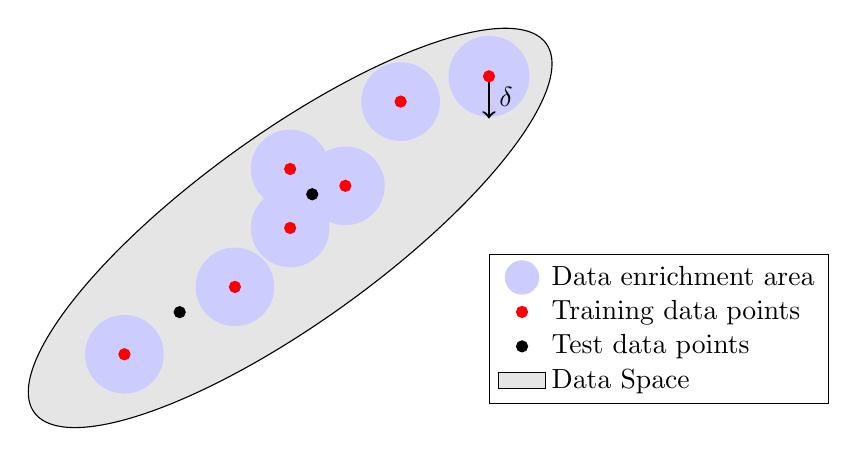
\begin{tikzpicture}
               \begin{axis}[
                xlabel={X-axis label},
                ylabel={Y-axis label},
                width=10cm,
                height=8cm,
                grid=major,
                legend style={at={(.8,.3)},anchor= west, nodes={right}},
                xmin=-3, xmax=3,
                ymin=-3, ymax=3,
                hide axis,
                ]
               \addplot[only marks, mark=*, mark options={scale=7, fill=blue!20, draw=blue!20}, forget plot] coordinates {
                (0,.7)
                (1,1.5)
                (0,0)
                (0.5,0.5)
                (-0.5,-0.7)
                (-1.5,-1.5)
                };
               \addplot[only marks, mark=*, mark options={scale=3, fill=blue!20, draw=blue!20}] coordinates {
                (0,0)
                };
               \addlegendentry{Data enrichment area}
               \addplot[only marks, color=red, mark=*] table [row sep=crcr] {
                x y \\
                0 .7 \\
                1 1.5 \\
                0 0 \\
                .5 .5 \\
                -.5 -.7 \\
                -1.5 -1.5 \\
                1.8 1.8 \\
                };
               \addlegendentry{Training data points}
               \addplot[only marks, color=black, mark=*] table [row sep=crcr] {
                x y \\
                0.2 .4 \\
                -1 -1 \\
                };
               \addlegendentry{Test data points}
               \addplot [
                domain=0:360,
                samples=100,
                smooth,
                variable=\t,
                fill=gray!20,
                forget plot,
                ] (
                {3.2 * cos(\t) * cos(45) - 1 * sin(\t) * sin(45)},
                {3.2 * cos(\t) * sin(45) + 1 * sin(\t) * cos(45)}
                );
               \addlegendimage{area legend, fill=gray!20, draw=black}
               \addlegendentry{Data Space}
               \begin{scope}
               \draw[thick, fill=blue!20, color = blue!20] (axis cs:1.8, 1.8) circle (.5cm);
               \draw[->, thick, black] (axis cs:1.8,1.8) -- (axis cs:1.8,1.3) node[midway, right] {$\delta$};
               \end{scope}
               \end{axis}
               \end{tikzpicture}
        }
        
    \end{column}
    \begin{column}{0.5\textwidth}
        2. Inducing implicit regularization terms, we simultaneously minimize 

        \[\MSE{\Psi{}|_{\ub^{i}} - \mc{F}|_{\ub^{i}}}\] 

        \[  \MSE{\nabla_{\ub}\Psi|_{\ub^{i}} - \nabla_{\ub}\mc{F}|_{\ub^{i}}} \]

        \[  \MSE{\nabla_{\ub}^2\Psi|_{\ub^{i}} - \nabla_{\ub}^2\mc{F}|_{\ub^{i}}} \]

    \end{column}
\end{columns}

}
% \myblue{Improve stability, long-term prediction capacity, and generalization.}

}

}
% \frame{
\frametitle{Prediction Error Estimation}
% \vspace{-9ex}
\small
% \bluebox{Two main benifits}
{

We define the error of the surrogate model $\ut{i}$ and true solutions $\ui{i}$ at certain time step $i$ as 

\vspace{-1ex}

\[\eg{i} = \MSE{\ut{i} - \ui{i}}.\]

\vspace{-1ex}

\begin{theorem}
    \theolab{mainTheo}
    Assume that the second derivative of $\F\LRp{\ub}$ with respect to $\ub$ is uniformly bounded.
    Let
    \[
        {f^{i+1}} := \dt\MSE{\F\LRp{\ut{i}} - \Psi\LRp{\ut{i}}},
    \]
    and
    \[
        {g^{i+1}} :=  \dt \MSE{\eval{\nabla_{\ub}\F}_{\ut{i}} -  \eval{\nabla_{\ub}\Psi}_{\ut{i}}} + \MSE{\mathbf{I} + \dt \eval{\nabla_{\ub}\Psi}_{\ut{i}}} + {c^i},
    \]
    where $c^i = \mc{O}\LRp{\eg{i}}$. Then,
    the prediction error $\eg{n}$ at time $t_n$ satisfies
    \[
        \eg{n} \le \sum_{k = 1}^{n}\LRp{\prod_{i = k+1}^{n}g^i} f^k.
    \]
\end{theorem}

}
% \myblue{Improve stability, long-term prediction capacity, and generalization.}

}

}
% \frame{
\frametitle{Motivation for \texttt{DGNet}}
\vspace{-10ex}
\bluebox{\texttt{mcTangent} uses fully connected neural network which}
{
\begin{itemize}
    \item cannot capture spatial correlation efficiently.
    \item only works for smooth solution problems.
\end{itemize}
}

}}
% \frame{
\frametitle{A Dual mesh - Discontinuous Galerkin \& Graph Neural Network}

}}
% \frame{
\frametitle{Schematic of \texttt{DGNet}}
\vspace{-2ex}
% \small
% \bluebox{Key idea}
{\small \texttt{DGNet} surrogate model is trained with 2nd-order strong stability preserving Runge-Kutta scheme.}
\vspace{1ex}
{

\def\layersep{2.cm}
\def\nodeinlayersep{.8cm}
\usetikzlibrary{calc}

% \raggedleft
% \centering
\resizebox{0.72\textwidth}{!}{
    \begin{tikzpicture}[
        node distance=\layersep,
        edge/.style={-stealth,shorten >=1pt, draw=black!50,thin, rounded corners=5pt},
        edge2/.style={draw=black!50,thin},
        neuron/.style={circle,fill=black!25,minimum size=10pt,inner sep=0pt},
        operator/.style={rectangle,fill=green!,minimum height= \nodeinlayersep, minimum width= 1.2 * \layersep, inner sep=0pt, rounded corners},
        input neuron/.style={neuron, fill=green!50,minimum size=12pt},
        output neuron/.style={neuron, fill=green!50,minimum size=12pt},
        hidden neuron/.style={neuron,,draw=blue,thick fill=blue!5},
        Forward map/.style={operator, fill=red!50},
        annot/.style={text width=4em, text centered},
        every node/.style={scale=1.0},
        node1/.style={scale=2.0},
        cross/.style={path picture={ 
            \draw[black, shorten <=2pt, shorten >=2pt, line width=1pt] 
                (path picture bounding box.south) -- (path picture bounding box.north); 
            \draw[black, shorten <=2pt, shorten >=2pt, line width=1pt] 
                (path picture bounding box.west) -- (path picture bounding box.east);
        }}
    ]
    
    \node[rectangle,fill=yellow!50,minimum height= \nodeinlayersep, minimum width= 1.2 * \layersep, rounded corners] (u_in) at (3.5*\layersep, -.00*\nodeinlayersep) {$\ubr^{i} = \ui{{i,0}} + \epsb$};
    
    % DG GNN RHS tikz figure
    \node[rectangle,draw=blue,thick,fill=blue!40,minimum height= \nodeinlayersep, minimum width= 1.2 * \layersep, rounded corners] (DGGNN-1) at (1*\layersep, -2*\nodeinlayersep) {$\DGGNN$};
    \node[rectangle,fill=yellow!50,minimum height= \nodeinlayersep, minimum width= 1.2 * \layersep, rounded corners] (SL-DGGNN-1) at (1*\layersep, -4.8*\nodeinlayersep) {$S$};
    \node[rectangle,fill=yellow!50,minimum height= \nodeinlayersep, minimum width= 1.2 * \layersep, rounded corners] (DGGNN-RK-1) at (1*\layersep, -6.5*\nodeinlayersep) {$\ut{{i},1}$};
    \node [draw,circle,cross,minimum width=.02*\layersep,line width=.3pt](cross_1) at (1*\layersep, -3.6*\nodeinlayersep){};
    \node[rectangle,minimum height= \nodeinlayersep, minimum width= 1.2 * \layersep, rounded corners] (dt) at (1.2*\layersep, -2.9*\nodeinlayersep) {\tiny $ \times \dt$};
    
    \draw[edge,thin] (u_in) -- (1*\layersep, -.00 *\nodeinlayersep) -- (DGGNN-1);
    \draw[edge,thin] (1*\layersep, -0.6 *\nodeinlayersep) -- (1*\layersep, -1 *\nodeinlayersep) -- (2*\layersep, -1 *\nodeinlayersep) -- (2*\layersep, -3.6 *\nodeinlayersep) -- (cross_1);
    \draw[edge,thin] (DGGNN-1) -- (cross_1);
    \draw[edge,thin] (cross_1) -- (SL-DGGNN-1);
    \draw[edge,thin] (SL-DGGNN-1) -- (DGGNN-RK-1);
    
    \node[rectangle,draw=blue,thick,fill=blue!40,minimum height= \nodeinlayersep, minimum width= 1.2 * \layersep, rounded corners] (DGGNN-2) at (1*\layersep, -8.5*\nodeinlayersep) {$\DGGNN$};
    \node[rectangle,fill=yellow!50,minimum height= \nodeinlayersep, minimum width= 1.2 * \layersep, rounded corners] (SL-DGGNN-2) at (1*\layersep, -11.6*\nodeinlayersep) {$S$};
    \node[rectangle,fill=yellow!50,minimum height= \nodeinlayersep, minimum width= 1.2 * \layersep, rounded corners] (DGGNN-RK-2) at (1*\layersep, -13.3*\nodeinlayersep) {$\ut{{i},2}$};
    \node [draw,circle,cross,minimum width=.02*\layersep,line width=.3pt](cross_2) at (1*\layersep, -10.1*\nodeinlayersep){};
    \node[rectangle,minimum height= \nodeinlayersep, minimum width= 1.2 * \layersep, rounded corners] (dt) at (1.2*\layersep, -9.4*\nodeinlayersep) {\tiny $ \times \dt$};
    \node[rectangle,minimum height= \nodeinlayersep, minimum width= 1.2 * \layersep, rounded corners] (dt) at (1.2*\layersep, -10.6*\nodeinlayersep) {\tiny $ \times \frac{1}{2}$};
    
    \draw[edge,thin] (DGGNN-RK-1) -- (DGGNN-2);
    \draw[edge,thin] (1*\layersep, -7.*\nodeinlayersep) -- (1*\layersep, -7.5*\nodeinlayersep) -- (2*\layersep, -7.5 *\nodeinlayersep) -- (2*\layersep, -10.1 *\nodeinlayersep) -- (cross_2);
    \draw[edge,thin] (DGGNN-2) -- (cross_2);
    \draw[edge,thin] (cross_2) -- (SL-DGGNN-2);
    \draw[edge,thin] (SL-DGGNN-2) -- (DGGNN-RK-2);
    
    \draw[edge,thin] (1*\layersep, -.6 *\nodeinlayersep) -- (1*\layersep, -1 *\nodeinlayersep) -- (0.*\layersep, -1 *\nodeinlayersep) -- (0.*\layersep, -10.1 *\nodeinlayersep) -- (cross_2);
    
    % DG solver RHS tikz figure
    \node[rectangle,fill=red!50,minimum height= \nodeinlayersep, minimum width= 1.2 * \layersep, rounded corners] (DGsol-1) at (6*\layersep, -2*\nodeinlayersep) {$\mc{F}$};
    \node[rectangle,fill=yellow!50,minimum height= \nodeinlayersep, minimum width= 1.2 * \layersep, rounded corners] (SL-DGsol-1) at (6*\layersep, -4.8*\nodeinlayersep) {$S$};
    \node[rectangle,fill=yellow!50,minimum height= \nodeinlayersep, minimum width= 1.2 * \layersep, rounded corners] (DGsol-RK-1) at (6*\layersep, -6.5*\nodeinlayersep) {$\ubar{{i},1}$};
    \node [draw,circle,cross,minimum width=.02*\layersep,line width=.3pt](cross_3) at (6*\layersep, -3.6*\nodeinlayersep){};
    \node[rectangle,minimum height= \nodeinlayersep, minimum width= 1.2 * \layersep, rounded corners] (dt) at (6.2*\layersep, -2.9*\nodeinlayersep) {\tiny $ \times \dt$};
    
    \draw[edge,thin] (u_in) -- (6*\layersep, -.00 *\nodeinlayersep) -- (DGsol-1);
    \draw[edge,thin] (6*\layersep, -.6 *\nodeinlayersep)  -- (6*\layersep, -1 *\nodeinlayersep) -- (5*\layersep, -1 *\nodeinlayersep) -- (5*\layersep, -3.6 *\nodeinlayersep) -- (cross_3);
    \draw[edge,thin] (DGsol-1) -- (cross_3);
    \draw[edge,thin] (cross_3) -- (SL-DGsol-1);
    \draw[edge,thin] (SL-DGsol-1) -- (DGsol-RK-1);
    
    \node[rectangle,fill=red!50,minimum height= \nodeinlayersep, minimum width= 1.2 * \layersep, rounded corners] (DGsol-2) at (6*\layersep, -8.5*\nodeinlayersep) {$\mc{F}$};
    \node[rectangle,fill=yellow!50,minimum height= \nodeinlayersep, minimum width= 1.2 * \layersep, rounded corners] (SL-DGsol-2) at (6*\layersep, -11.6*\nodeinlayersep) {$S$};
    \node[rectangle,fill=yellow!50,minimum height= \nodeinlayersep, minimum width= 1.2 * \layersep, rounded corners] (DGsol-RK-2) at (6*\layersep, -13.3*\nodeinlayersep) {$\ubar{{i},2}$};
    \node [draw,circle,cross,minimum width=.02*\layersep,line width=.3pt](cross_4) at (6*\layersep, -10.1*\nodeinlayersep){};
    \node[rectangle,minimum height= \nodeinlayersep, minimum width= 1.2 * \layersep, rounded corners] (dt) at (6.2*\layersep, -9.4*\nodeinlayersep) {\tiny $ \times \dt$};
    \node[rectangle,minimum height= \nodeinlayersep, minimum width= 1.2 * \layersep, rounded corners] (dt) at (6.2*\layersep, -10.6*\nodeinlayersep) {\tiny $ \times \frac{1}{2}$};
    
    \draw[edge,thin] (DGsol-RK-1) -- (DGsol-2);
    \draw[edge,thin] (6*\layersep, -7.*\nodeinlayersep) -- (6*\layersep, -7.5*\nodeinlayersep) -- (5*\layersep, -7.5 *\nodeinlayersep) -- (5*\layersep, -10.1 *\nodeinlayersep) -- (cross_4);
    \draw[edge,thin] (DGsol-2) -- (cross_4);
    \draw[edge,thin] (cross_4) -- (SL-DGsol-2);
    \draw[edge,thin] (SL-DGsol-2) -- (DGsol-RK-2);
    
    \draw[edge,thin] (6*\layersep, -.6 *\nodeinlayersep) -- (6*\layersep, -1 *\nodeinlayersep) -- (7.*\layersep, -1 *\nodeinlayersep) -- (7.*\layersep, -10.1 *\nodeinlayersep) -- (cross_4);
    
    \node[rectangle,fill=green!40,minimum height= \nodeinlayersep, minimum width= 1.6 * \layersep, rounded corners] (loss_mc) at (3.5*\layersep, -9.5*\nodeinlayersep) {\begin{tabular}{c} Loss  $\mc{L}_{mc}$: \vspace*{.2cm} \\  $\MSEdg{\ubar{{i},1} - \ut{{i},1}}$ \vspace*{.2cm} \\ $ + $ \vspace*{.2cm} \\ $ \MSEdg{\ubar{{i},2} - \ut{{i},2}}$ \end{tabular}};
    
    \draw[edge,thin] (DGGNN-RK-1) -- (3.5*\layersep, -6.5 *\nodeinlayersep) -- (loss_mc);
    \draw[edge,thin] (DGGNN-RK-2) -- (3.5*\layersep, -13.3 *\nodeinlayersep) -- (loss_mc);
    
    \draw[edge,thin] (DGsol-RK-1) -- (3.5*\layersep, -6.5 *\nodeinlayersep) -- (loss_mc);
    \draw[edge,thin] (DGsol-RK-2) -- (3.5*\layersep, -13.3 *\nodeinlayersep) -- (loss_mc);
    
    
    
    % ML loss  term 
    \node[rectangle,fill=green!40,minimum height= \nodeinlayersep, minimum width= 1.6 * \layersep, rounded corners] (loss_ml) at (-2.*\layersep, -9.5*\nodeinlayersep) {\begin{tabular}{c} Loss $\mc{L}_n$: \vspace*{.2cm} \\  $\MSEdg{\ui{{i},1} - \ut{{i},1}}$ \vspace*{.2cm} \\ $ + $ \vspace*{.2cm} \\ $ \MSEdg{\ui{{i},2} - \ut{{i},2}}$ \end{tabular}};
    
    \draw[edge2,thin] (DGGNN-RK-1) -- (.08*\layersep, -6.5 *\nodeinlayersep)
        arc [start angle=0, end angle=180, radius=0.08*\layersep] 
        -- (-1.*\layersep, -6.5 *\nodeinlayersep);
    \draw[edge,thin] (-1.*\layersep, -6.5 *\nodeinlayersep) -- (-2.*\layersep, -6.5 *\nodeinlayersep) -- (loss_ml);
    \draw[edge,thin] (DGGNN-RK-2) -- (-2.*\layersep, -13.3 *\nodeinlayersep) -- (loss_ml);
    
    % Pre-computed data
    \node[rectangle,fill=gray!40,minimum height= \nodeinlayersep, minimum width= 1.6 * \layersep, rounded corners] (data_set) at (-2.1*\layersep, 1.2*\nodeinlayersep) {\begin{tabular}{c} Pre-computed data \vspace*{.2cm} \\  $\ui{i,0}, \ui{i,1}, \ui{i,2}$ \end{tabular}};
    \draw[edge,thin] (data_set) -- (-2.1*\layersep, -7.58 *\nodeinlayersep);
    
    \draw[edge,thin] (data_set) -- (3.45*\layersep, 1.2 *\nodeinlayersep) -- (3.45*\layersep, .5 *\nodeinlayersep);
    
    % Randomize machine engine
    \node[rectangle,fill=gray!40,minimum height= \nodeinlayersep, minimum width= 1.6 * \layersep, rounded corners] (random_noise_engine) at (6*\layersep, 1.2*\nodeinlayersep) {\begin{tabular}{c} Random noise \vspace*{.2cm} \\  $\epsb \sim \mc{N} \LRp{\mathbf{0}, \delta^2 \LRs{\boldsymbol{\diag}\LRp{{\ui{i,0}}}}^2}$ \end{tabular}};
    \draw[edge,thin] (random_noise_engine) -- (3.55*\layersep, 1.2 *\nodeinlayersep) -- (3.55*\layersep, .5 *\nodeinlayersep);
    
    \end{tikzpicture}
}

}

}}
% \frame{
\frametitle{Numerical Results - Airfoil}
\vspace{-2ex}
\small
\bluebox{2D Euler Equations}
{
    % Use the flalign environment which allows for left alignment
\begin{flalign*}
&\frac{\partial}{\partial t}
\begin{pmatrix}
\rho \\
\rho u \\
\rho v \\
E
\end{pmatrix}
+ \frac{\partial}{\partial x_1}
\begin{pmatrix}
\rho u \\
\rho u^2 + p \\
\rho u v \\
u(E + p)
\end{pmatrix}
+ \frac{\partial}{\partial x_2}
\begin{pmatrix}
\rho v \\
\rho u v \\
\rho v^2 + p \\
v(E + p)
\end{pmatrix} = 0, &
\end{flalign*}

\vspace{-3ex}

\begin{flalign*}
&E = \frac{p}{\gamma - 1} + \frac{\rho}{2} \left(u^2 + v^2 \right). &
\end{flalign*}


\text{with the initial conditions}
\begin{flalign*}
&\rho_0 = \gamma, \rho_0 u_0 = M \gamma, \rho_0 v_0 = 0, p_0 = 1, E_0 = \frac{p_0}{\gamma - 1} + \frac{\rho_0}{2}\left(u_0^2 + v_0^2\right) &
\end{flalign*}

}

\orangebox{Data generation}
{
    \begin{itemize}
        \item Training data: Mach $M = 0.8$, $\gamma = \left \{1.2, 1.6 \right \}$, $AoA = 3^o$, $T = [0,1.2]s$
        \item Test data: \quad \, Mach $M = 1.2$,  \,$\gamma = 1.4$, \quad \, \quad \,$AoA = 5^o$, $T = [0,7.5]s$
    \end{itemize}
}
}}
% \frame{
\frametitle{Numerical Results - Airfoil}
\vspace{-2ex}
\small
% \bluebox{Key idea}
{

}

}}
% \frame{
\frametitle{Numerical Results - Double Mach Reflection}
\vspace{-2ex}
\small
% \bluebox{Key idea}
{

}

}}
% \frame{
\frametitle{Numerical Results - Out of Distribution Generalization}
\vspace{-2ex}
\small
% \bluebox{Key idea}
{

}

}}
% \frame{
\frametitle{Numerical results - Computational Cost}
\vspace{-2ex}
\small
% \bluebox{Key idea}
{

}

}}
% \frame{
\frametitle{Takeaways}
\vspace{-2ex}
\small
% \bluebox{Key idea}
{
\begin{itemize}
    \item \texttt{DGNet} 
\begin{itemize}
    \item is able to learn the dynamical evolution of shock-type problems.
    \item is able to generalize to out-of-distribution scenarios.
    \item provides an error estimation bound for predictions.
\end{itemize}
    % \item Data randomization technique induces regularizations + enriches training data information.

\end{itemize}

}

}
}


% \frame{
\frametitle{Model-constrained Machine Learning for Solving Inverse Problems}
% \vspace{-10ex}
\bluebox{I worked on}
{
\begin{itemize}
    \item \texttt{TNet} [\myblue{3}] - A model-constrained deep learning approach for solving inverse problems.
    \item \texttt{TAEN} [\myblue{4}] - A model-constrained Tikhonov autoencoder network for solving both forward and inverse problems. This is a significant improvement from \texttt{TNet} [\myblue{3}].
\end{itemize}
}
{ \tiny
[3] {\bf H.V. Nguyen}, et. al. {\it ``TAEN: A Model-Constrained Tikhonov Autoencoder Network for Forward and Inverse Problems."} Under
Review at  Computer Methods in Applied Mechanics and Engineering  (2025) \newline
[4] {\bf H.V. Nguyen}, et. al. {\it ``TNet: A Model-Constrained Deep Learning Approaches for Inverse Problems."} SIAM Journal of Scientific
Computing (2024)
}
}
}
% \input{\fromroot{slides/Inverse_challenges.tex}}
% \input{\fromroot{slides/Inverse_surrogates.tex}}
% \frame{
\frametitle{Problem settings}
\small
\vspace{-3ex}
\bluebox{}
{
We consider 
\begin{itemize}
    \item The forward problem
    \begin{equation*}
        \yb = B \circ \underbrace{G (\ub)}_{\omb} + \, \delta,
    \end{equation*}
    where $B$ is observational operator, $G$ is forward map, and $\delta$ is white noise. 
    
    \item The equivalent inverse problem
    \begin{equation*}
        \ub = \LRp{B \circ G}^\dagger \yb = {\GB}^\dagger \yb.
    \end{equation*}
\end{itemize}
}

\vspace{5ex}

\bluebox{}
{
    {\bf Task: }Given the observation data $\yb$, we want to learn autoencoder surrogate models 
\begin{itemize}
    \item Encoder $\Psie(\yb)$ for inverse map ${\GB}^\dagger$.
    \item Decoder $\Psid(\ub)$ for forward map $G$.
\end{itemize}
}

}
}
% \input{\fromroot{slides/Inverse_mc_AE_scheme_phase_1.tex}}
% \input{\fromroot{slides/Inverse_mc_AE_scheme_phase_1_cont.tex}}
% \input{\fromroot{slides/Inverse_mc_AE_scheme_phase_2.tex}}
% \input{\fromroot{slides/Inverse_mc_AE_scheme_phase_2_cont.tex}}
% \input{\fromroot{slides/Inverse_TAEN.tex}}
% \frame{
\frametitle{TAEN: Tikhonov Autoencoder Network}
\vspace{-2ex}

{\small

\begin{corollary}
Given \myblue{\bf $\bar{Y}$ is a full row rank} training data, for a test observation sample $\ybtest$, the predicted \texttt{TAEN} inverse solution is
\begin{equation*}
    \ub^{\TNetAE} = \Psie^*(\ybtest) = \LRp{ \Ib + \lambda {\GB}^T \GB }^{-1} \LRp{ \ub_0 + \lambda {\GB}^T \ybtest}
\end{equation*}
which is exactly the inverse solution of the following linear Tikhonov regularization problem
\begin{equation*}
    \min_{\ub}  \halfv{1} \nor{\ub - \ub_0}_{2}^2 + \halfv{\lambda} \nor{\GB \ub - \ybtest}_{2}^2.
\end{equation*}
Then, the \myred{test inverse solution error}
\[
    \epsb_{\ubtest}^{\TNetAE} = \nor{\Psie^*(\ybtest) - \ubtest }_2^2 \leq  \nor{{\ub^\text{test} - {\ub}_0} }_2^2
\]        
Meanwhile, for a test parameter $\ubtest$, the \myred{test forward solution error}
\[
    \epsb_{\ybtest}^{\TNetAE} = \nor{\Psid^*(\ubtest) - \ybtest }_2^2  = 0,
\]
\end{corollary}
}
}}
% \input{\fromroot{slides/Inverse_mc_AE_Y_full_row_rank.tex}}
% \input{\fromroot{slides/Inverse_numerical_heat_1.tex}}
% \input{\fromroot{slides/Inverse_numerical_heat_2.tex}}
% \input{\fromroot{slides/Inverse_numerical_heat_3.tex}}
% \input{\fromroot{slides/Inverse_numerical_heat_4.tex}}
% \input{\fromroot{slides/Inverse_numerical_NS_1.tex}}
% \input{\fromroot{slides/Inverse_numerical_NS_2.tex}}
% \input{\fromroot{slides/Inverse_numerical_NS_3.tex}}
% \input{\fromroot{slides/Inverse_numerical_NS_4.tex}}
% \input{\fromroot{slides/Inverse_numerical_computational_cost.tex}}
% \input{\fromroot{slides/Inverse_conclusion.tex}}



% \frame{
\frametitle{DIAS: Data-informed Active Subspace Regularization Framework for Solving Inverse Problems}
% \vspace{-10ex}
% \bluebox{}
% {
% I proposed data-informed active subspace regularization framework for solving inverse problems.
% }

\vspace{3ex}

{ \tiny
[6] {\bf H.V. Nguyen}, et. al. {\it ``A Data-Informed Active Subspace Regularization Framework for Inverse Problems."} Computation (2022)
}

}}
% \frame{
\frametitle{Motivation}
\vspace{-5ex}
\bluebox{Solving inverse problems}
{
Given the observation $\yb$ and a linear forward model $G$, we infer for parameter $\ub$ by solving

\[\ub^* = \min_{\ub} \,
\half \nor{G\ub - \yb}_{\ycovinv}^2\]

However, the inverse problem is usually ill-posed including instability, non-uniqueness, non-existence. A widely-used remedy is to regularize the parameter by a prior term, e.g., Tikhonov regularization framework, as following 

\[\ub^* = \min_{\ub} \, \half \nor{G\ub - \yb}_{\ycovinv}^2  + \halfv{\lambda} \nor{\ub}_{\ucovinv}^2 \]

\myred{The key issue: we essentially regularize the whole parameter space.} Ideally, only unimportant subspace, which causes instability, should be regularized.   

}


}}
% \frame{
\frametitle{Methodology}
\vspace{-1ex}
\bluebox{DIAS key steps}
{
\begin{enumerate}
    \item Finding the inactive subspace. 
    
    \begin{itemize}
        \item We define a function 
    
        \[f(\ub) = \nor{G\ub - \yb}_{\ycovinv}^2\]

        \item Calculate the covariance matrix 
        
        \[
        C = \int \nabla_{\ub} f(\ub) \LRp{\nabla_{\ub} f(\ub)}^T \rho(\ub) d\ub, \quad \quad \rho(\ub) \sim \mc{N}\LRp{\ub_0, \Gamb}
        \]
        \item Eigen-decomposition of $C$ for active subspace $\W_1$  and inactive subspace $\W_2$.
    \vspace{-2ex}
    \[ C = \W D \W^T \quad \implies \quad \LRs{\W_1 \, \W_2} = \LRs{\underbrace{\W[:r]}_{\text{top r}} \quad \underbrace{\W[r:]}_{\text{remaining}}} \]
    \end{itemize}
    \vspace{-4ex}
    \item Solving the the optimization problem
    \[\ub^* = \min_{\ub} \, \half \nor{G\ub - \yb}_{\ycovinv}^2  + \halfv{\lambda} \nor{\W_2^T \ub}_{\LRp{\W_2^T \Gamb \W_2}^{-1}}^2 \]
\end{enumerate}
}

}}
% \frame{
\frametitle{Numerical results - X-ray tomography inverse problem}
\vspace{-4ex}
\bluebox{Why don't we use SVD of $G$ for unimportant modes of parameter $\ub$?}
{

\begin{figure}[htb!]
    \centering
    % \caption{{\bf 2D heat equation.} A (random) representative case of inverse and full forward solution obtained by $\TNetAE$ trained with 1 training sample coupled with data randomization of noise level $\sigma = 0.1$. $\TNetAE$ inverse solution is comparable to the Tikhonov (Tik) inverse counterpart, and both are consistent with the ground truth (True). $\TNetAE$ full forward solution is almost identical (in fact within 3 digits of accuracy) to the underlying true solution.}
    \resizebox{\textwidth}{!}{
    \begin{tabular*}{\textwidth}{c@{\hskip 0.4cm} c@{\hskip 0.4cm} c@{\hskip 0.4cm}}
        \centering
        \raisebox{-0.5\height}{1st eigenvector of $G$} &
        \raisebox{-0.5\height}{1st eigenvector of AS} &
        \raisebox{-0.5\height}{true parameter $\ub$}
        \\ ~\\
        \raisebox{-0.5\height}{\includegraphics[width = 0.3\textwidth]{Figs/Figs/DIAS/EigenV_1.pdf}} &
        \raisebox{-0.5\height}{\includegraphics[width = 0.3\textwidth]{Figs/Figs/DIAS/EigenW_1.pdf}} &
        \raisebox{-0.5\height}{\includegraphics[width = 0.3\textwidth]{Figs/Figs/DIAS/X_ray_True.pdf}}
    \end{tabular*}
    }
\end{figure}

}

}}
% \frame{
\frametitle{Numerical results - X-ray tomography inverse problem}
\vspace{-4ex}
% \bluebox{Why don't we use SVD of $G$ for unimportant modes of parameter $\ub$?}
{
\begin{figure}[htb!]
    \centering
    % \caption{{\bf 2D heat equation.} A (random) representative case of inverse and full forward solution obtained by $\TNetAE$ trained with 1 training sample coupled with data randomization of noise level $\sigma = 0.1$. $\TNetAE$ inverse solution is comparable to the Tikhonov (Tik) inverse counterpart, and both are consistent with the ground truth (True). $\TNetAE$ full forward solution is almost identical (in fact within 3 digits of accuracy) to the underlying true solution.}
    \resizebox{1\textwidth}{!}
    {
    \begin{tabular*}{\textwidth}{c c@{\hskip 0.2cm} c@{\hskip 0.2cm} c@{\hskip 0.2cm} c@{\hskip 0.2cm}}
        \centering
        &
        \raisebox{-0.5\height}{under regularization} &
        \raisebox{-0.5\height}{optimal regularization} &
        \raisebox{-0.5\height}{over regularization} &
        \raisebox{-0.5\height}{True } 
        \vspace{-1ex}
        \\
        \vspace{1ex}
        &
        \raisebox{-0.5\height}{small $\lambda$} &
        \raisebox{-0.5\height}{optimal $\lambda$} &
        \raisebox{-0.5\height}{very large $\lambda$} &
        \\ 
        \rotatebox[origin=c]{90}{Tikhonov} &
        \raisebox{-0.5\height}{\includegraphics[width = 0.21\textwidth]{Figs/Figs/DIAS/X_ray_Tikhonov_alpha_001.pdf}} &
        \raisebox{-0.5\height}{\includegraphics[width = 0.21\textwidth]{Figs/Figs/DIAS/X_ray_Tikhonov_alpha_13.pdf}} &
        \raisebox{-0.5\height}{\includegraphics[width = 0.21\textwidth]{Figs/Figs/DIAS/X_ray_Tikhonov_alpha_10000.pdf}} &
        \raisebox{-0.5\height}{\includegraphics[width = 0.21\textwidth]{Figs/Figs/DIAS/X_ray_True.pdf}}
        \vspace{1ex}
        \\
        \rotatebox[origin=c]{90}{AS} &
        \raisebox{-0.5\height}{\includegraphics[width = 0.21\textwidth]{Figs/Figs/DIAS/X_ray_ACT_Full_r_10000_alpha_001.pdf}} &
        \raisebox{-0.5\height}{\includegraphics[width = 0.21\textwidth]{Figs/Figs/DIAS/X_ray_ACT_Full_r_10000_alpha_13.pdf}} &
        \raisebox{-0.5\height}{\includegraphics[width = 0.21\textwidth]{Figs/Figs/DIAS/X_ray_ACT_Full_r_10000_alpha_10000.pdf}} &
    \end{tabular*}
    }
\end{figure}

}

}}
% \frame{
\frametitle{Takeaways}
\vspace{-5ex}
\bluebox{DIAS}
{
\begin{itemize}
    \item is robust with large range of regularization parameter $\lambda$, thus avoid tuning $\lambda$.
    \item is applicable to non-linear inverse problems.
\end{itemize}
}

}}



% \frame{
\frametitle{Collaborated work}
\vspace{-1ex}
\bluebox{I worked on other projects}
{
\begin{itemize}
    \item Developed a {\bf data-informed active subspace regularization framework} for solving inverse problems [\myblue{6}]. In DIAS, the observation data informs the active subspace of PoI. We keep this active subspace intact from regularization, thus achieving better inverse solutions compared to Tikhonov regularization framework.
    \item Developed {\bf model-Constrained machine learning approaches for solving Bayesian inverse problems} [\myblue{5}]. We aim to develop a real-time uncertainty qualification approach for inverse problems. This work was built upon the \texttt{TNet} [\myblue{4}].
    \item {\bf Unifying randomized methods for inverse problems} [\myblue{7}]. We unified different randomized methods for solving inverse problems under the same umbrella and thus providing a guideline for discovering new randomization methods.
\end{itemize}
}

% \vspace{1ex}

{ \tiny
[4] {\bf H.V. Nguyen}, et. al. {\it ``TNet: A Model-Constrained Deep Learning Approaches for Inverse Problems."} SIAM Journal of Scientific
Computing (2024) \newline
[5] R.S. Philley, {\bf H.V. Nguyen}, et. al. {\it ``Model-Constrained Empirical Bayesian Neural Networks for Inverse Problems."} XLIV
Ibero-Latin ACCME (2023) \newline
[6] {\bf H.V. Nguyen}, et. al. {\it ``A Data-Informed Active Subspace Regularization Framework for Inverse Problems."} Computation (2022) \newline
[7] J. Wittmer, {\bf H.V. Nguyen}, et. al. {\it ``On Unifying Randomized Methods for Inverse Problems."} Inverse Problems (2023)
}

}}



% \frame{
\frametitle{Proposed research (ongoing)}
\vspace{-20ex}
\bluebox{[1] Model-constrained machine learning for varying observations inverse problem (with Ali)}
{
    Upon the success of \texttt{TAEN} and \texttt{TNet}, I have been working on developing model-constrained machine learning approaches for solving inverse problems with varying observations.
}





% \vspace{3ex}

% \bluebox{Designing transformer architecture}
% {
%     Upon the success of \texttt{DGNet} and \texttt{mcTangent}, I have been working on designing new transformer architecture for solving PDEs / physics time-series data prediction problems.
% }

}}
% \frame{
\frametitle{Proposed research (ongoing)}
\vspace{-20ex}
\bluebox{[2] Designing transformer architecture (with Son, Venu)}
{
    Upon the success of \texttt{DGNet} and \texttt{mcTangent}, I have been working on designing new transformer architecture for solving PDEs / physics time-series data prediction problems.
}





% \vspace{3ex}

% \bluebox{Designing transformer architecture}
% {
%     Upon the success of \texttt{DGNet} and \texttt{mcTangent}, I have been working on designing new transformer architecture for solving PDEs / physics time-series data prediction problems.
% }

}}



% \input{\fromroot{slides/thesis_statement_future.tex}}








% \input{\fromroot{slides/Inverse_inverse_and_forward_problems.tex}}
% \input{\fromroot{slides/Inverse_challenges.tex}}
% \input{\fromroot{slides/Inverse_surrogates.tex}}
% \input{\fromroot{slides/Inverse_linear_settings.tex}}
% \input{\fromroot{slides/Inverse_all_AE.tex}}
% \input{\fromroot{slides/Inverse_naive_AE.tex}}
% \input{\fromroot{slides/Inverse_mc_AE_scheme_phase_1.tex}}
% \input{\fromroot{slides/Inverse_mc_AE_scheme_phase_1_cont.tex}}
% \input{\fromroot{slides/Inverse_mc_AE_scheme_phase_2.tex}}
% \input{\fromroot{slides/Inverse_mc_AE_scheme_phase_2_cont.tex}}
% \input{\fromroot{slides/Inverse_mc_AE.tex}}
% \input{\fromroot{slides/Inverse_mc_AE_cont.tex}}
% \input{\fromroot{slides/Inverse_TAEN.tex}}
% \input{\fromroot{slides/Inverse_mc_AE_Y_full_row_rank.tex}}
% \input{\fromroot{slides/Inverse_comparison_all_approaches.tex}}
% \input{\fromroot{slides/Inverse_numerical_results_overal.tex}}
% \input{\fromroot{slides/Inverse_numerical_heat_1.tex}}
% \input{\fromroot{slides/Inverse_numerical_heat_2.tex}}
% \input{\fromroot{slides/Inverse_numerical_heat_3.tex}}
% \input{\fromroot{slides/Inverse_numerical_heat_4.tex}}
% \input{\fromroot{slides/Inverse_numerical_NS_1.tex}}
% \input{\fromroot{slides/Inverse_numerical_NS_2.tex}}
% \input{\fromroot{slides/Inverse_numerical_NS_3.tex}}
% \input{\fromroot{slides/Inverse_numerical_NS_4.tex}}
% \input{\fromroot{slides/Inverse_numerical_computational_cost.tex}}
% \input{\fromroot{slides/Inverse_conclusion.tex}}
\end{document}